\documentclass[a4paper]{report}
\title{Frequency Domain Adaptive Receiver Design for OFDM Modulation}
\author{Kevin Exton \\Supervisor: Dr. Gayathri Kongara}
\date{\today}
\newcommand{\tabitem}{~~\llap{\textbullet}~~}
\usepackage{hyperref}
\usepackage{amsmath}
\usepackage[section]{placeins}
\usepackage{cite}
\usepackage[parfill]{parskip}
\usepackage{caption}
\usepackage{subcaption}
\usepackage{graphicx}
\usepackage{amssymb}
\usepackage{mathrsfs}
\usepackage{rotating}
\usepackage{pdfpages}
\usepackage{minted}
\usepackage[toc,page]{appendix}
\usepackage[margin=1.1in]{geometry}
\renewcommand{\bibname}{References}
\begin{document}
\maketitle
\renewcommand{\abstractname}{Executive Summary}
\newpage
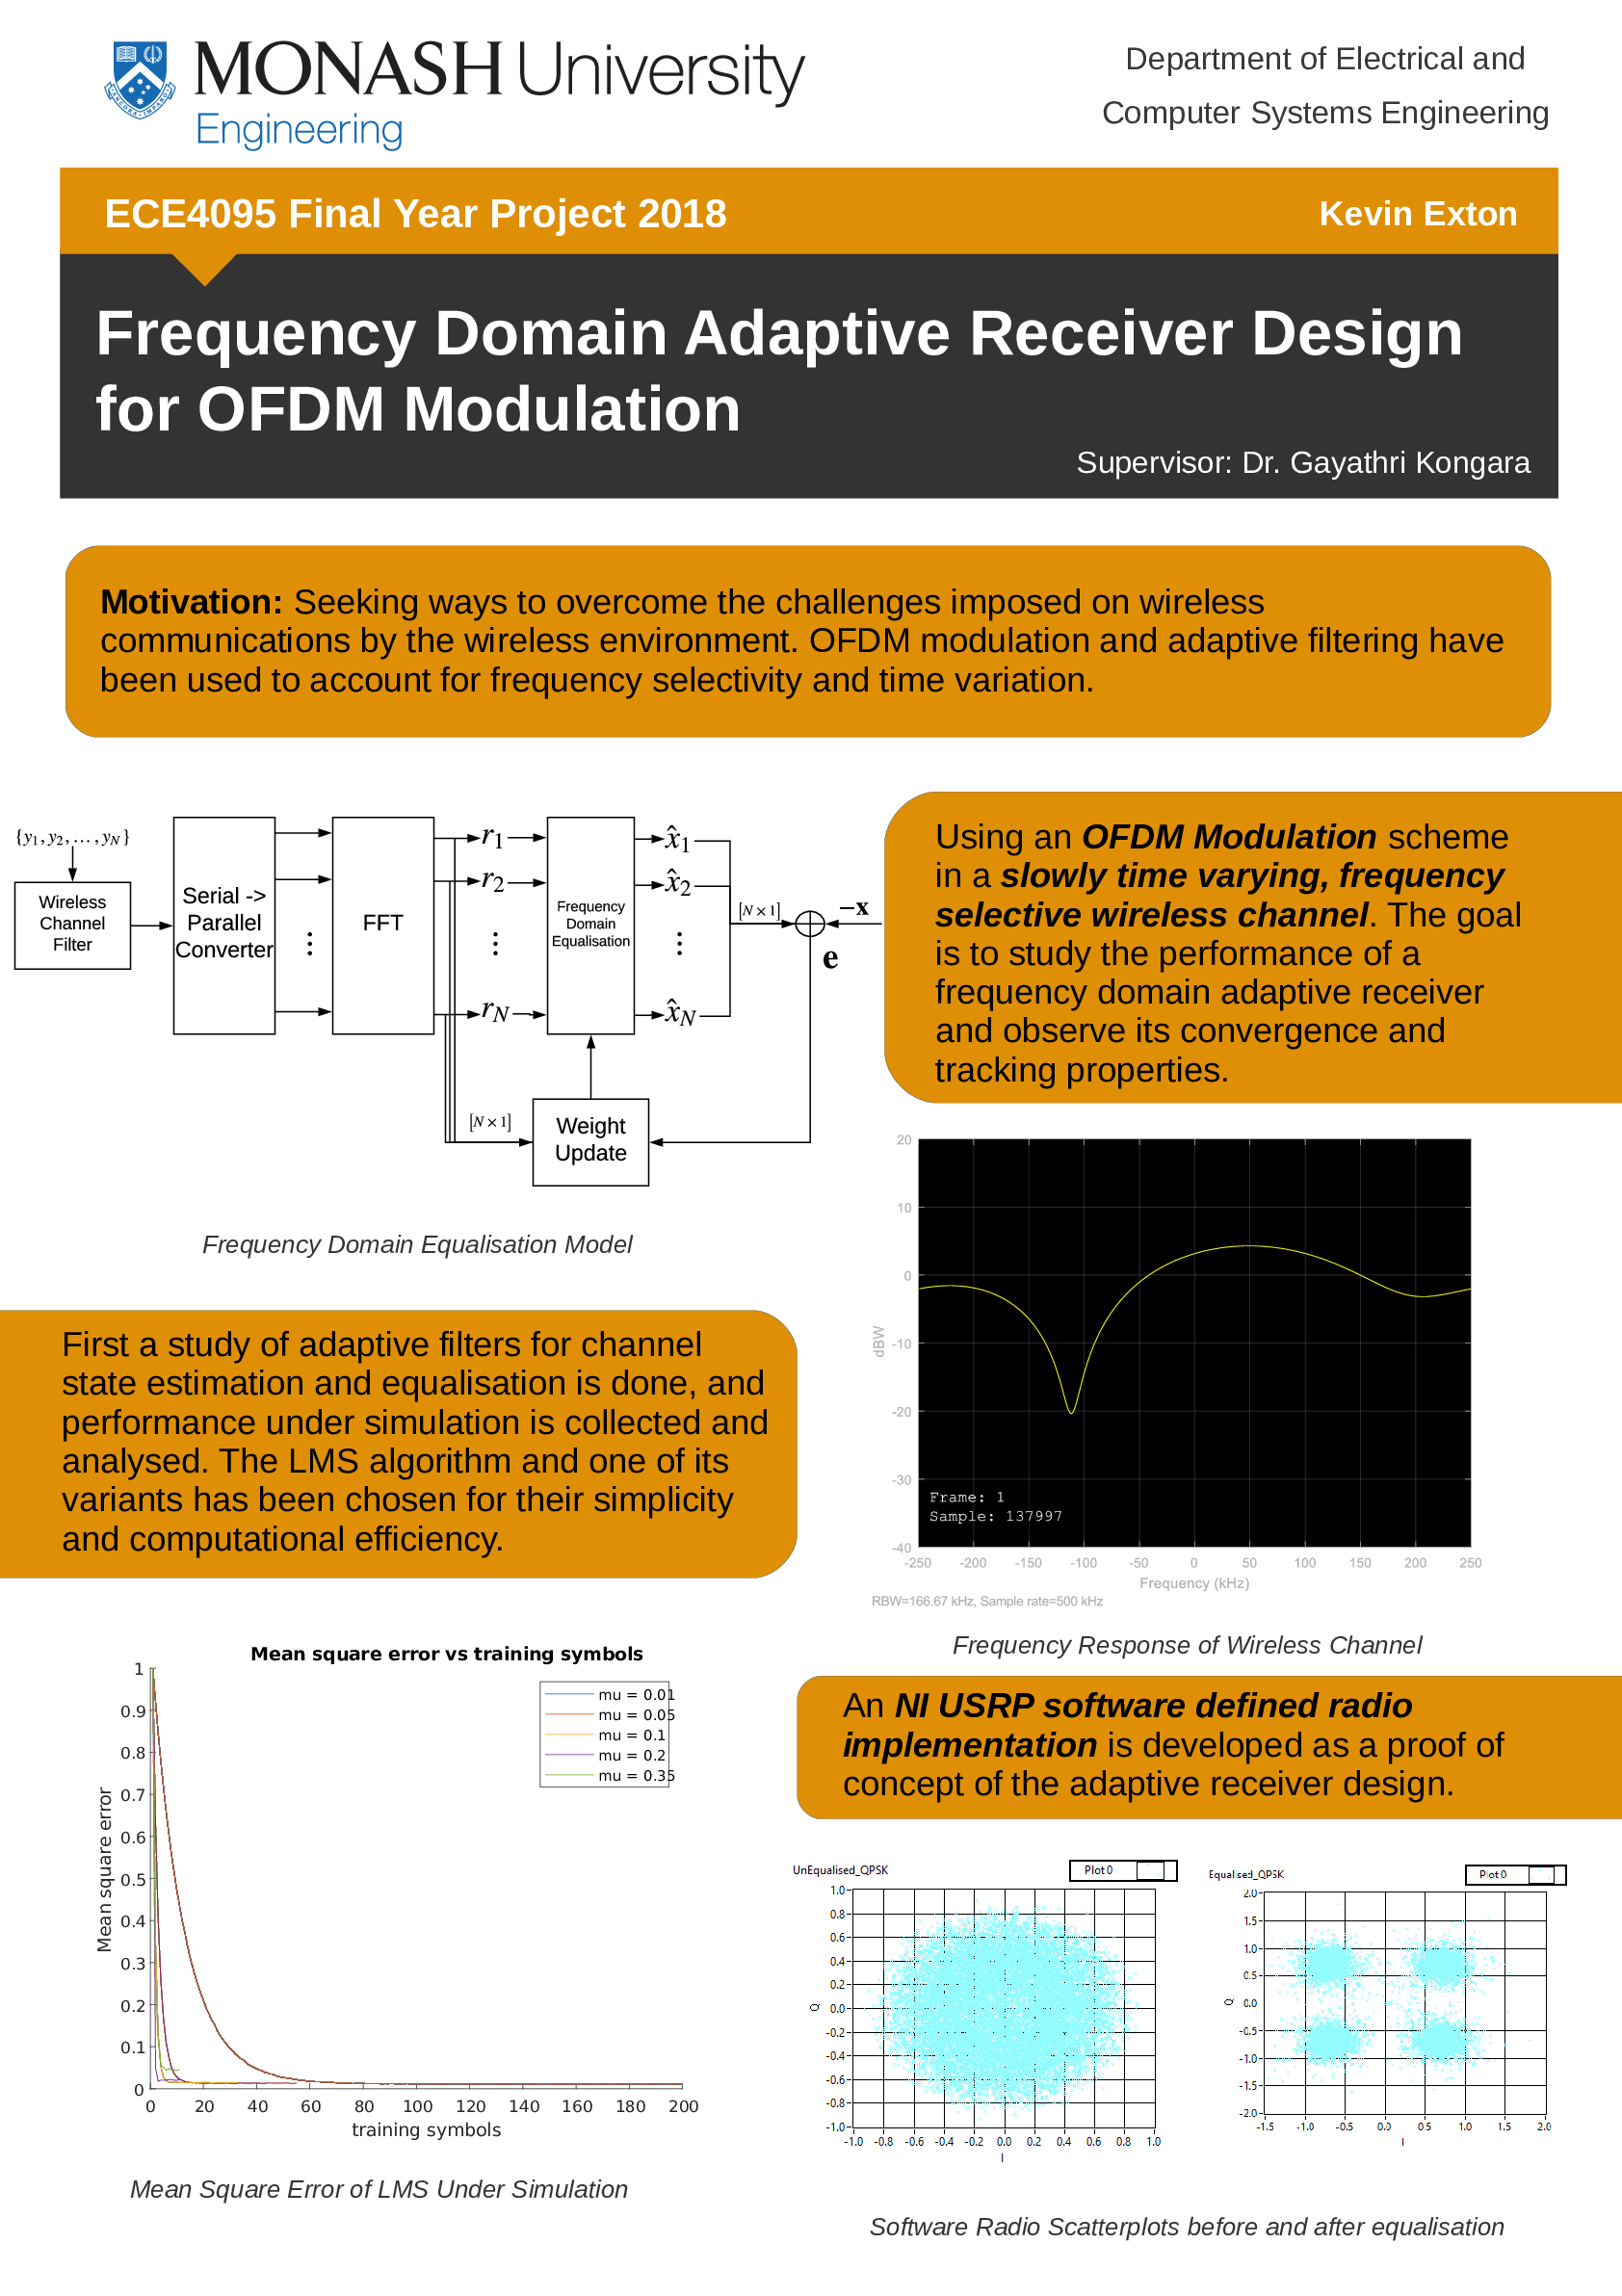
\includepdf{./Figures/Poster/KevinPoster2.png}
\newpage
\pagenumbering{gobble}
\section*{Significant Contributions}
Studied adaptive filter theory in order to design and prototype %
a hardware implementation of a frequency domain adaptive equaliser %
for OFDM modulation. The hardware prototype was developed on the %
National Instruments universal software radio platform model 2943R.
\begin{figure*}[ht]
	\centering
	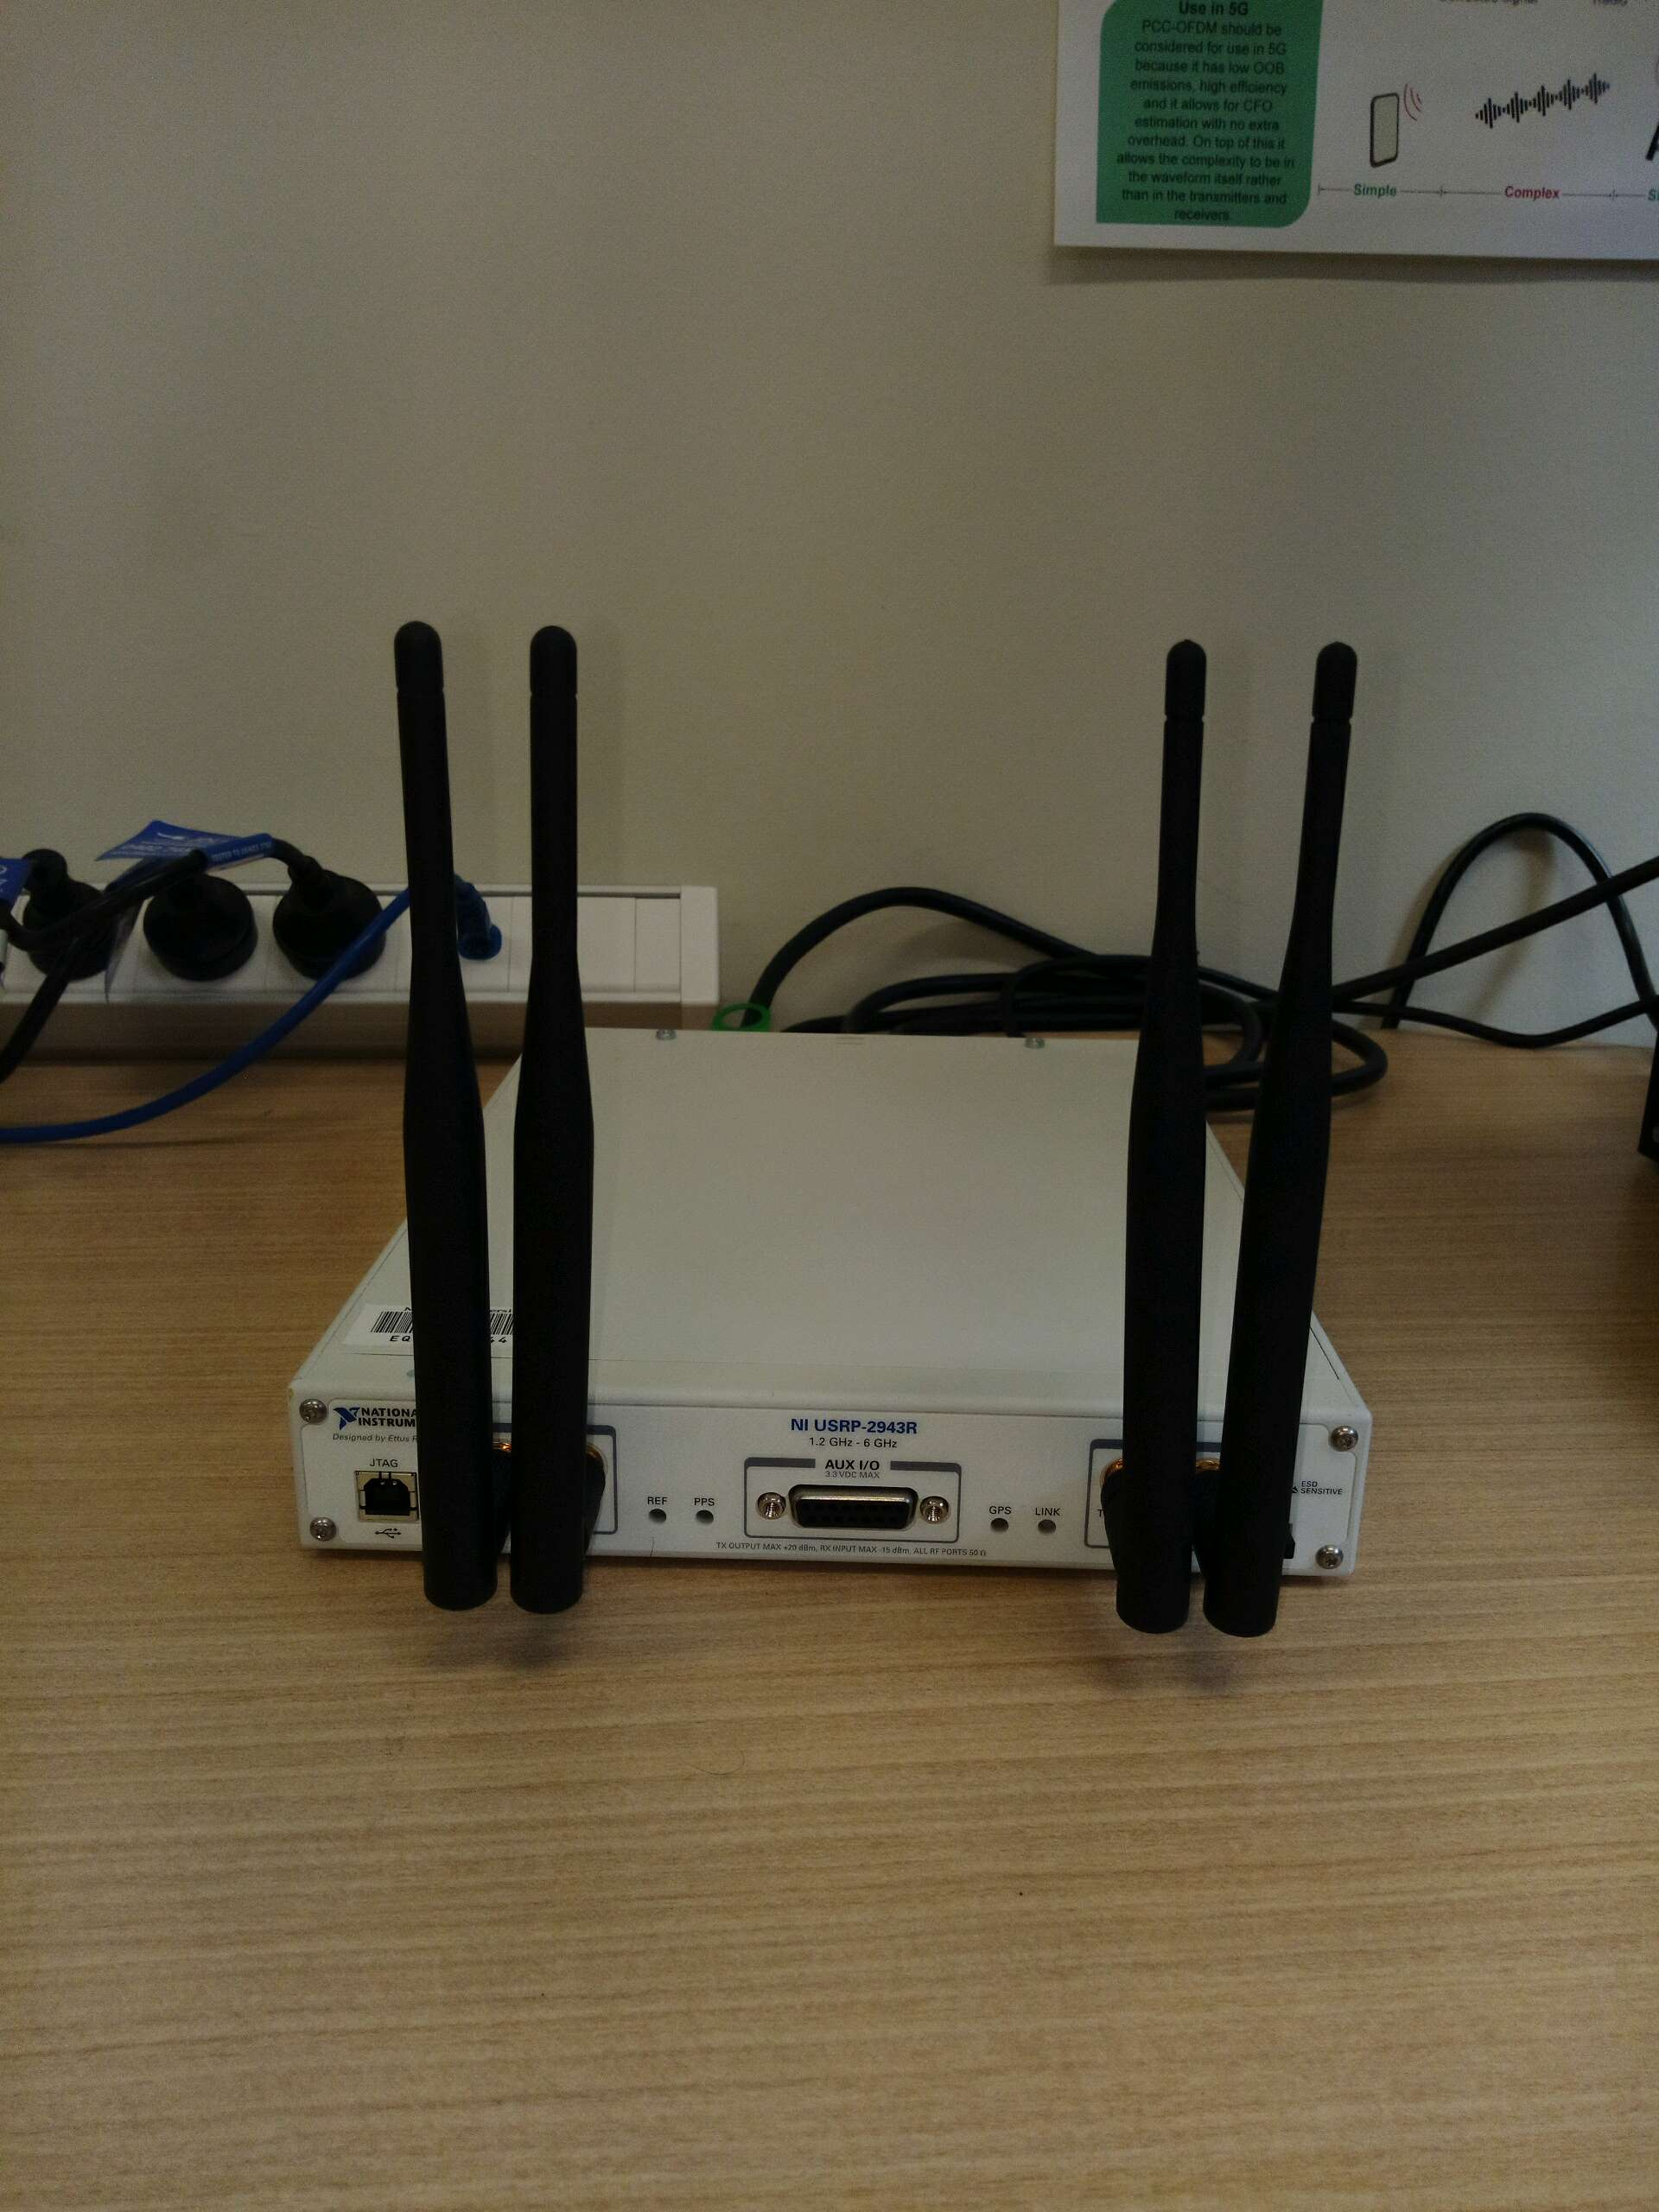
\includegraphics[width=0.5\textwidth]{./Figures/%
	SignificantContributions/Radio.jpg}
	\caption*{USRP-2943R}
\end{figure*}
\section*{Simulation code repository:}
\url{https://github.com/kcexn/FYP-Simulation}
\begin{abstract}
Real wireless channels we may wish to communicate over %
are often frequency selective and time varying. The rate %
at which the channel varies and the extent to which it %
is frequency selective may greatly limit valid choices of %
signal bandwidth. Orthogonal Frequency Division Multiplexing %
(OFDM) has become a popular modulation scheme in wireless %
communication in large part due to the fact that the overall %
bandwidth of the OFDM symbol and the bandwidth of the %
subcarriers within the OFDM symbol can be decoupled overcoming %
challenges related to frequency selectivity of the wireless channel. %
The time varying nature of the wireless channel still poses a significant %
challenge to successful communication however. This study %
looks at two adaptive equalisation schemes that can track %
the changes in the channel state over time in the frequency %
domain to work with OFDM, the least mean square (LMS) %
filter and the normalised least mean square filter (NLMS). As the %
coherence time of the channel reduces, the faster the channel %
changes with time and the more difficult it is to track with %
adaptive equalisation, as such, this study constrains itself to %
only slowly time varying scenarios where adaptive equalisation %
will track the changes in the channel state. A hardware implementation %
has been developed on the National Instruments universal software %
radio platform (USRP) to demonstrate the proof of concept.
\end{abstract}
\pagenumbering{arabic}
\tableofcontents
\chapter{Introduction}
\label{ch:Introduction}
\section{Motivating Scenario}
\label{sec:MotivatingScenario}
The next generation of wireless communication %
dubbed 5G makes promises of a hyper connected %
world with billions of devices coming online % TODO: cite this
connected by the radio network. With this kind %
of communication network in mind, it is easy %
to imagine a scenario in which a cell needs %
to serve many almost static users a steady stream %
of data over a long period of time.% 

\begin{figure}[h!]
	\includegraphics[width=\linewidth]{./Figures/%
	Application_Scenario.png}
	\caption{Application Scenario}
	\label{fig:AppScene}
\end{figure}

Figure \ref{fig:AppScene}. visualises the motivating %
scenario in mind of one base station serving many %
terminals over a bidirectional link. I'll be constraining %
% TODO: Add up-link study to the conclusion about future study
the study done within this report to simply the down-link % 
between the base station and a terminal. This link will %
have a few properties of interest to us. The first is that %
the terminal will be fairly static with very little movement, %
the second, is that the environment is prone to change. We can %
imagine this scenario as being a user, sitting down in a busy %
courtyard watching streaming video on their mobile phone. The %
user equipment is unlikely to move much however the environment %
connecting the user to the base station is prone to change as %
people and vehicles move about. I will model this environment %
as one that will introduce slow time-variations to the wireless %
% Find some examples or citations of this?
channel connecting the station to the user. No more time will be %
spent analysing the validity of this channel model as %
the key focus of this report will be to analyse the %
effectiveness of adaptive filters under these channel %
conditions.

With this scenario in mind this report will be broken %
into the following sections. The rest of this chapter %
will aim to introduce the topics of the wireless %
communication principles used throughout the rest %
of the report, adaptive filtering, orthogonal %
frequency division multiplexing, and wireless %
channel modeling will receive a high level treatment %
here. Chapter 2 will give OFDM a more in-depth %
mathematical discussion. % This will probably be very short
% but I can probably flesh it out if I give it some 
% comparison and look at OOB emissions and the such.
Chapter 3 will give adaptive filtering a similar %
in-depth mathematical treatment. Chapter 4 will study %
channel models and channel modeling techniques. %
Chapter 5 will develop my system model both under %
under simulation and on the software defined radio. %
Chapter 6 will look at the results under simulation %
both on the radio and in MATLAB. Chapter 7 will draw %
some conclusions and make some remarks about future %
directions that can be explored.

\section{Orthogonal Frequency Division Multiplexing %
(OFDM)}

The simplest way to modulate signals over the wireless %
channel is to use some form of single carrier modulation. %
Single carrier modulation simply takes input data, separates %
it into in-phase and quadrature components if necessary, pulse %
shapes the signal, up converts to the carrier frequency and %
transmits over the wireless channel.
%TODO: add figure to depict single carrier methodology

This method of modulation has some drawbacks. %TODO: find some 
% references that list some drawbacks of single carrier modulation.
The main drawbacks of interest to us will be the complexity of %
channel equalisation. The wireless propagation medium can be %
modeled as a finite impulse response filter %TODO: cite this
and so as the filter length increases estimating, %
the channel becomes an increasingly more complex task. %
A modulation technique that helps to overcome this challenge %
is orthogonal frequency division multiplexing or OFDM. %
OFDM works differently to traditional single carrier %
modulation in the sense that it separates the modulation %
bandwidth into $N$ subcarriers each with a subband bandwidth of %
$\frac{B_total}{N}$.

%TODO: add figure depicting the serial to parallel OFDM

A cyclic prefix can be added to the beginning of each OFDM %
symbol which gives it the nice mathematical properties %
which make equalisation simple regardless of the length %
of the channel filter. In addition, the parallel nature %
of the signal means that signal processing can happen %
on each subband independently and can reduce the bandwidth %
requirements for signal processing electronics.

The details of OFDM will be developed in Chapter 2. 
%TODO: fix chapter numbers
Where the mathematical construction of OFDM will be
explored as well as the nature of the cyclic prefix.

\section{Adaptive Filtering}

%TODO: Do some reading to find a good way to motivate Adaptive
% filters. Want to compare it to static filters at the 
% very least. Maybe even want to introduce some filter
% theory full stop.

\section{Channel Modeling}

%TODO: Do some reading to find a good way to motivate channel
% models. Want to introduce the wireless system model. And 
% connect the channel model to the idea of a filter. Connecting
% it to adaptive filtering and OFDM.


\chapter{Orthogonal Frequency Division Multiplexing}
\

\chapter{Wireless Channel Modeling}

% TODO: Introduce Fadnig impairments following
% Simulation of Communication Systems

% TODO: give the text book description of large scale fading
\newpage
\section{Fading Channels}

Fading is a major component of wireless channel %
impairments. Fading comes under two main categories %
large scale and small scale fading. Figure \ref{fig:Fading} %
illustrates these two main components of fading.
\FloatBarrier
\begin{figure}[h!]
	\centering
	\includegraphics[width=\textwidth,
		height=\textheight, keepaspectratio]
		{./Figures/%
		WirelessChannel/LargeandSmallScale%	
		Fading.png}
	\caption{combination of large and small %
		scale fading (a) and the small-scale %
		fading component (b) from %
		\cite{Sklar97-1}}
	\label{fig:Fading}
\end{figure}

\FloatBarrier
\subsection{Large Scale Fading}

Large scale fading, also sometimes referred to as %
shadow fading is characterised by an attenuation %
of the average signal power as can be seen in %
figure \ref{fig:Fading}a). It is caused %
by significant obstructions to the signal such as %
buildings or hills between the transmitter and %
receiver. The receiver is therefore being %
\emph{shadowed} by the obstruction. 

The received signal power can be modeled as:

\begin{align}
	S_{r} = S_{t} + G_{t} + G_{r} - L_{p}
\end{align}

Where $S_{r}$ is the received signal power in dB, %
$S_{t}$ is the transmit signal power in dB, $G_{t}$ 
and $G_{r}$ are the transmit and receive antenna %
gains in dB and $L_{p}$ is the propagation loss in dB. %
Typically $S_{r}$, $S_{t}$, $G_{t}$, and $G_{r}$ are %
either well known or are easily modeled, in the case of %
fading channels the propagation loss is the most difficult %
to predict \cite{Jer00}. There are two main methods %
of attempting to model $L_{p}$, ray tracing methods %
which must be location specific and statistical models. %
I will constrain this section to the development of %
statistical models. 

The most popular of the statistical models are the %
class of slope-intercept models \cite{Jer00}. These %
models treat propagation loss as being composed of %
a deterministic component and a statistical component.

\begin{align}
	L_{p} = \alpha + \beta log_{10}(R) + \gamma \text{ dB}
\end{align}

where $R$ is the distance from the transmitter to the %
receiver in kilometres, $\alpha$ and $\beta$ are parameters %
determined by the model, and $\gamma$ is the %
statistical component of the model. Values for $\alpha$ and %
$\beta$ are determined from experimental measurements %
where received signal power averaged over several %
wavelengths are taken over many different locations %
around the transmitter. These received signal %
powers can be plotted against the log of %
the distance to the transmitter and a least squares fit %
can be made to the data. The resulting residuals around %
the least squares fit describes $\gamma$.

Some well-known slope intercept models are the Hata%
\cite{Hata80} model and the COST-231 model\cite{COST231}.

Typically the residuals  of the slope intercept models %
when measured in dB follow a gaussian distribution with %
zero mean and a standard deviation of about 8dB\cite{Jer00}.
So the large scale fading follows a log-normal distribution.

\subsection{Small Scale Fading}

Small scale fading, also commonly referred to as multipath %
fading is caused by the transmitted signal following many %
different paths before arriving at the receiving antenna. %
Each of these multiple paths can have different lengths %
and may be reflected or refracted many times, a process %
typically referred to as scattering. As a result of the %
varying distances each propagation path takes, the time %
taken for a transmitted waveform to reach the receiver %
is also going to vary down each of these paths, figure %
\ref{fig:MultipathChannel} illustrates this multipath %
behaviour.

\begin{figure}[ht]
	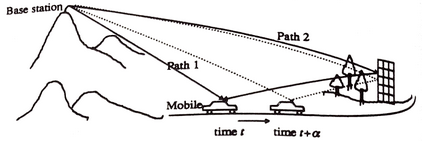
\includegraphics[width=\textwidth]{./Figures/%
		WirelessChannel/MultipathChannel.png}
	\caption{Multipath Channel \cite{Jer00}}
	\label{fig:MultipathChannel}
\end{figure} 

The resulting effect of this multipath channel is that %
symbols transmitted at different times will arrive %
at the receiver at the same time, this leads to %
a self-interfering effect that can cause the received %
signal power to undergo large fluctuations and can %
be characterised as inter-symbol interference.

The multipath fading can be broadly organised into %
two separate categories\cite{Jer00}.

\begin{enumerate}
	\item{The multipath signal paths are made up %
		of relatively small and identifiable number %
		of components reflected by small hills, %
		houses, and other strucutres encountered in %
		open areas and rural environments. This %
		results in a channel model with a finite number %
		of multipath components. Such a channel is %
		referred to as a \emph{discrete multipath channel}.}
	\item{The multipath signal paths are generated by %
		a large unresolvable reflections as might occur %
		in a mountainous area or in a dense urban environment. %
		This signal is composed of a continuum of %
		unresolvable multipath components. This %
		channel model is referred to as a \emph{diffuse %
		multipath channel}.}
\end{enumerate}

Multipath reflected components can be described in %
terms of orthogonal components $x_{n}(t)$ and %
$y_{n}$%
(t), where $x_{n}(t) + jy_{n}(t) = \alpha_{n}(t)e^{%
-j\theta_{n}(t)}$. If the number of random components %
is large enough and none are dominant, then the received %
components $x_{r}(t)$ and $y_{r}(t)$ which are the sums %
of the reflected signals will have a gaussian probability %
density function. The magnitude of the received scattered %
components will have a magnitude described by:

\begin{align}
	r_{0}(t) = \sqrt{x_{r}^{2}(t) + y_{r}^{2}(t)}
\end{align}

The probability density function of the envelope $r_{0}(t)$ %
of the received signal is going to follow a Rayleigh distribution %
with probability density function:

\begin{align}
	f_{R}(r_{0}) = \begin{cases}
		\frac{r_{0}}{\sigma^{2}}e^{-r_{0}^{2}/(2\sigma^{2})} %
		& \text{ for } r_{0} \geq 0 \\
		0 & \text{ otherwise}
	\end{cases}
	\label{eq:RayleighPDF}
\end{align}

Where $\sigma^{2}$ is the mean power of the received %
multipath signal. This type of fading is called Rayleigh %
fading.

\begin{figure}[h!]
	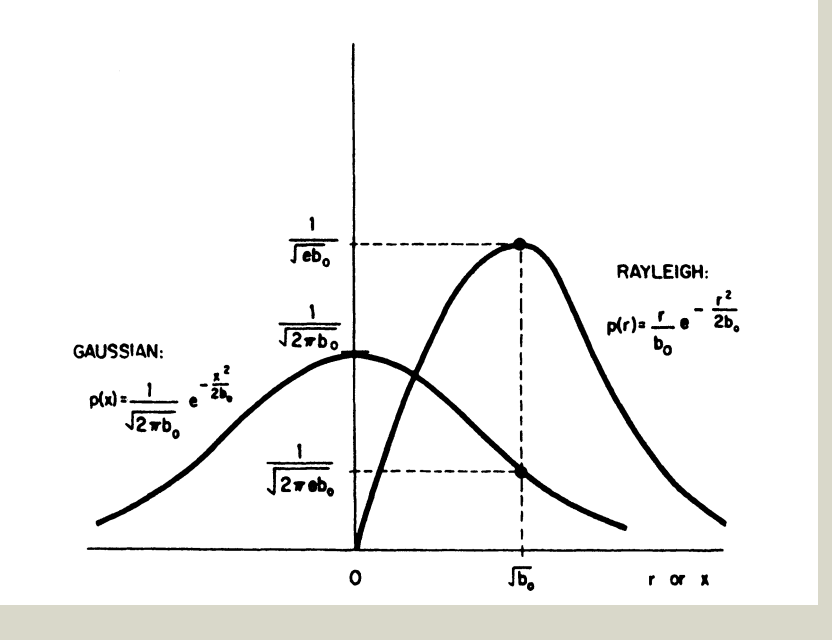
\includegraphics[width=\linewidth]{./Figures/%
	WirelessChannel/RayleighDistribution.png}
	\caption{Gaussian and Rayleigh Distributions%
	\cite{Jakes74}}
	\label{fig:RayleighDistribution}
\end{figure}

Figure \ref{fig:RayleighDistribution} illustrates %
the gaussian distribution and the rayleigh %
distribution.

When the received signal is made up of multiple %
reflected rays and a significant line-of-sight %
component, the received envelope ampliude %
follows a Rician distribution with probability density %
function:

\begin{align}
	f_{R}(r_{0}) = \begin{cases}
		\frac{r_{0}}{\sigma^{2}}I_{0}%
		\left[ \frac{A_{r}}{\sigma^{2}} \right]%
		e^{-(r_{0}^{2}-A^{2})/(2 \sigma^{2})}%
		 & \text{ for } r_{0} \geq 0, A \geq 0\\
		0 & \text{ Otherwise}
	\end{cases}
	\label{eq:RicianPDF}
\end{align}

where $I_{0}$ is the modified zeroth order %
bessel function of the first kind. This kind of %
fading is commonly referred to as Rician fading. %
The Rician distribution is commonly described in %
terms of a parameter K\cite{Sklar01}, which is defined as %
the ratio of power in the specular component to the %
power in the multipath signal and is given as:

\begin{align}
	K = \frac{A^{2}}{2\sigma^{2}}
\end{align}

Figure \ref{fig:RicianDistribution} illustrates the relationship %
of the rician probability density function to the rayleigh %
PDF with respect to mean specular signal amplitude $v$ and %
mean scattered signal power of $1$.

\begin{figure}[ht]
	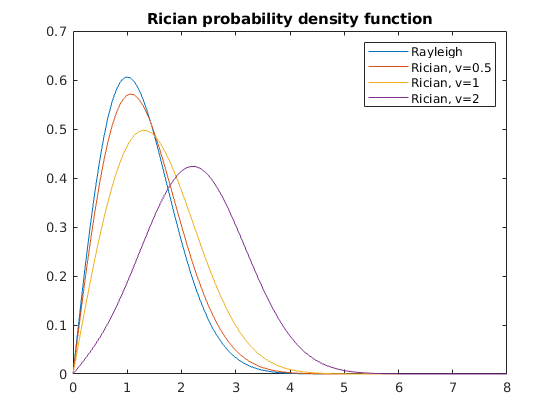
\includegraphics[width=\linewidth]{./Figures/%
	WirelessChannel/RicianDistribution.png}
	\caption{Rayleigh and Rician Probability %
	Density Function}
	\label{fig:RicianDistribution}
\end{figure}

\section{Time and Frequency Characteristics of Fading %
Channels}

% TODO: find and plot a measured Rayleigh distribution

\section{Wireless Channel as a Filter}

Good modeling and simulation of this small scale fading %
is crucial to the accurate simulation of wireless channels. %
There are two main methods of simulating small scale fading, %
the sums of sinusoids method first developed by Jakes in %
\cite{Jakes74} and a filtered white gaussian noise method. %
The filtered white gaussian noise methodology is the chosen %
method of simulation for this report.



% TODO: Develop Finite impulse response filter model 
% of the wireless channel

% TODO: develop the model for the time-varying characteristics
% of wireless channels

% TODO: Develop the mathematics of the finite gaussian channel model



\chapter{Adaptive Filtering}
\label{chap:AdaptiveFiltering}
The previous chapter on wireless channel modeling established %
the wireless channel as a type of FIR filter. The aim of the %
receiver is to undo the effects of the channel filter. %
Figure \ref{fig:CommSysModel}. shows the communications %
system model as described in \cite{Sklar01}, for this section %
we'll draw our attention to the section of the model beginning %
at pulse modulation and ending at detection. 
\begin{figure}[ht]
	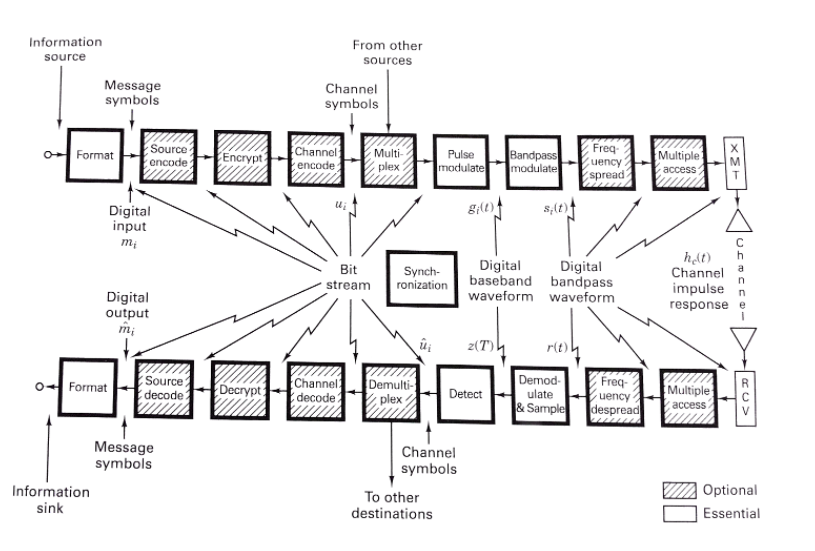
\includegraphics[width=\linewidth]{./Figures/Adaptive%
		Filters/CommunicationsSystemModel.png}
	\caption{Communications System Model \cite{Sklar01}}
	\label{fig:CommSysModel}
\end{figure}
The wireless system transfer function can be defined as:
\begin{align}
	H(f) = H_{t}(f)H_{c}(f)H_{r}(f)
\end{align}
where $H_{t}$ is the transfer function of the transmit filter, 
defined in the pulse modulate block, %
$H_{c}(f)$ is the transfer function of the channel, and $H_{r}%
(f)$ is the transfer function of the receive filter, defined in %
the demodulate and sample block. It's clear from this %
expression that the received baseband symbols at the %
detect block will be distorted by the channel filter $H_{c}%
(f)$, the goal of equalisation is to define an equalisation %
transfer function $H_{e}(f)$ that removes the effect of %
the channel filter. Such that the new system transfer %
function looks like this:
\begin{align}
	H(f) = H_{t}(f)H_{c}(f)H_{r}(f)H_{e}(f)
\end{align}
where
\begin{align}
	H_{c}(f)H_{e}(f) = 1
\end{align}
Throughout this entire chapter my development of adaptive filters %
will quite closely follow \cite{Hay02}. I'll start by %
developing the zero-forcing solution and the minimum mean square %
error solution also known as the Wiener solution. I'll then develop %
the stochastic gradient and the least mean square solution. A brief %
development of the recursive least square will be covered here as %
well.

\section{A Static Filter and The Wiener Solution}
% Need to introduce this section
\subsection{A Simple Filter the Zero-Forcing Solution}
\label{subsec:ZeroForcing}
Previously in chapter \ref{chap:OFDM} on OFDM, a key insight to %
the advantage of using the DFT was that the circular convolution %
in combination with the convolution theorem provided the nice %
property that the distortion introduced by the FIR channel filter %
introduced in chapter \ref{chap:ChannelModeling} can be represented %
as element wise multiplication in the frequency domain (see equation %
\ref{eq:DFTConvolutionTheorem}). It's clear that equation %
\ref{eq:ZeroForcing} does in fact represent a filtering operation %
in the frequency domain. This simple filter is commonly known as %
the zero forcing filter and is defined as the reciprocal of the %
frequency response of the channel filter $\frac{1}{H(f)}$. %
It's most easily found when a known set of symbols $X[i]$ have %
been transmitted such that
\begin{align}
	H\left[i\right] = \frac{Y\left[i\right]}{X\left[i\right]}
\end{align}
In a noiseless and time invariant environment this is the optimal %
solution to the equalisation problem. However a more accurate %
model for the received samples $y[nT]$ is
\begin{align}
	y[nT]=h[nT]\circledast x[nT]%
	+ v
\end{align}
where $h[nT]$ represents the channel filter of length %
$\mu$ at time $nT$ and $x[nT]$ are the inputs to %
$h[nT]$, $v$ represents the additive white gaussian %
noise (AWGN). Taking the DFT of both sides gives %
\begin{align}
	Y[i] = H[i]X[i] + V[i]%
	,\quad \text{ for } i = 0,1,\cdots,N-1
	\label{eq:AWGNModel}
\end{align}
Where $N$ is the length of the DFT. It's clear from %
equation \ref{eq:AWGNModel} that dividing through %
by $X[i]$ gives a noisy estimate of the channel %
frequency response
\begin{align}
	\frac{Y[i]}{X[i]} = H[i] + \frac{V[i]}{X[i]}, %
	\text{ for } i = 0,1,\cdots,N-1
\end{align}
equalising using this expression will lead to estimates %
of $X$
\begin{align}
	\hat{X}[i] =& \frac{H[i]X[i]+V[i]}{H[i]+V[i]/X[i]} \\
	=& \frac{H[i]X[i]}{H[i]+V[i]/X[i]} + \frac{V[i]}{H[i]
	+ V[i]/X[i]} \\
	=& \frac{H[i]}{H[i]+V[i]/X[i]}X[i] + 
	\frac{V[i]X[i]}{H[i]X[i]+V[i]}\\
	=& \frac{H[i]}{H[i]+V[i]/X[i]}X[i] + 
	\frac{V[i]X[i]}{Y[i]}
	\label{eq:NoiseAmplification}
\end{align}
Should $X[i]/Y[i]$ in equation \ref{eq:NoiseAmplification} %
be greater than $1$ then the noise in the received estimate %
$\hat{X}[i]$ will be amplified reducing SNR and increasing the bit %
error rate (BER).

\subsection{The Wiener Solution}
A solution to the noise amplification problem seen in %
section \ref{subsec:ZeroForcing} is to find the optimal %
solution taking noise into consideration. It's clear that %
this problem can be framed as an optimisation problem %
and so a measure of performance or cost function must %
first be defined to optimise. A natural choice for cost function %
is that of the mean square value of the estimation error. This %
is because the mean square error criterion results in a %
second order dependence for the cost function on the %
unknown coefficients in the impulse response of %
the filter. This leads to the cost function having a distinct %
minimum that uniquely defines the optimum %
statistical design of the filter \cite{Hay02}.
\subsubsection{The Wiener-Hopf Equations}
To develop this optimum solution first we revisit equation %
\ref{eq:BasebandChannelFIR} which describes the wireless channel %
as an FIR filter and for consistency with \cite{Hay02} and %
with my later development on my system model redefine it as
\begin{align}
	u(n) = \sum_{i}\tilde{h}(\tau)\tilde{s}(t-\tau)
	\label{eq:ChannelOut}
\end{align}
where $u(n)$ are now the series of inputs to an optimally %
designed filter with form shown in equation \ref{eq:FilterOut}. %
For the purposes of this chapter %
we will assume that the channel is time-invariant and set %
$\tilde{h}(\tau;t)$ to $\tilde{h}(\tau)$.
\begin{align}
	y(n) = \sum_{k=0}^{N-1}w_{k}^{*}u(n-k), n - 0,1,2,\cdots,N-1
	\label{eq:FilterOut}
\end{align}
where $y(n)$ is the output of the equalising filter, %
$u(n-k)$ are the discrete samples being received %
after having been distorted by the wireless channel, %
$w_{k}^{*}$ are the %
filter coefficients and the asterisk $^*$ represents %
complex conjugation. The estimation error will be defined as 
\begin{align}
	e(n) = d(n) - y(n)
	\label{eq:EstimationError}
\end{align}
where $d(n)$ is the desired output of the filter %
hence the %
mean square error criterion will be defined as
\begin{align}
	J =& E\left[e(n)e^{*}(n)\right]
	\label{eq:MeanSquareError}\\
	=& E\left[\lvert e(n) \rvert^{2}\right]
\end{align}
where $E\left[\cdot\right]$ denotes the expectation %
operator. With these definitions in mind the aim is now %
to minimise $J$. To do this the complex derivative of $J$ with %
respect to the filter coefficients $w_{k}^{*}$ needs %
to be found. First we'll define
\begin{align}
	w_{k}^{*} = a_{k} + jb_{k}
\end{align}
and 
\begin{align}
	\nabla_{k} = \frac{\partial}{\partial a_{k}} + j 
	\frac{\partial}{\partial b_{k}}
\end{align}
where $\nabla_{k}$ is the complex derivative %
operator with respect to $w_{k}^{*}$. From %
equations \ref{eq:FilterOut}, \ref{eq:EstimationError} %
and \ref{eq:MeanSquareError} %
\begin{align}
	\nabla_{k}J =& E\left[ \frac{\partial e(n)}
	{\partial a_{k}} e^{*}(n) + \frac{\partial
	e^{*}(n)}{\partial a_{k}}e(n) + \frac{
	\partial e(n)}{\partial b_{k}}je^{*}(n) 
	+ \frac{\partial e^{*}(n)}{\partial b_{
	k}}je(n)\right] \label{eq:DerivativeJ}
\end{align}
When evaluated 
\begin{align}
	\nabla_{k}J = -2E\left[u(n-k)e^{*}(n)\right]
	\label{eq:CostDerivative}
\end{align}
Since the mean square error criterion is quadratic %
the optimum solution can be found at its stationary %
point by setting
\begin{align}
	\nabla_{k}J =& 0,\quad\text{ for } k=0,1,2,\cdots,N-1
\end{align}
which implies that
\begin{align}
	E\left[u(n-k)e^{*}(n)\right] = 0,\quad\text{ for } k = 0,1,2,\cdots,N-1
	\label{eq:OptimalityCondition}
\end{align}
substituting equation \ref{eq:EstimationError} into %
\ref{eq:OptimalityCondition} gives
\begin{align}
	E\left[u(n-k)\left(d^{*}(n) - \sum_{m=0}^{N-1}w_{o_{m}}u
	^{*}(n-m)\right)\right]=0,\quad\text{ for }k=0,1,\cdots,N-1
\end{align}
where $w_{o_{m}}$ is the $m\text{th}$ coefficient of %
the impulse response of the optimum filter. Expanding and %
rearranging
\begin{align}
	&E\left[u(n-k)d^{*}(n) - u(n-k)\sum_{m=0}^{N-1}w
	_{o_{m}}u^{*}(n-m)\right] = 0\\
	\implies &E\left[u(n-k)d^{*}(n)\right] - E\left[u(n-k)\sum
	_{m=0}^{N-1}w_{o_{m}}u^{*}(n-m)\right] = 0\\
	\implies &E\left[u(n-k)d^{*}(n)\right] - \sum_{m=0}^{N-1}
	w_{o_{m}}E\left[u(n-k)u^{*}(n-m)\right] = 0\\
	\implies &E\left[u(n-k)d^{*}(n)\right] = 
	\sum_{m=0}^{N-1}w_{o_{m}}E\left[u(n-k)u^{*}(
	n-m)\right],\quad\text{for }k=0,1,\cdots,N-1
	\label{eq:ExpandedOptimalityCondition}
\end{align}
The expectation on the right side of equation %
\ref{eq:ExpandedOptimalityCondition} is the %
\emph{autocorrelation function} of the filter input %
for a lag of $m-k$ and can be expressed as
\begin{align}
	r(m-k) = E\left[u(n-k)u^{*}(n-m)\right]
	\label{eq:WienerAutocorrelation}
\end{align}
The expectation on the left side of equation %
\ref{eq:ExpandedOptimalityCondition} is the %
\emph{cross correlation} between the filter %
input and the desired response for a lag %
of $-k$ and can be expressed as
\begin{align}
	p(-k) = E\left[u(n-k)d^{*}(n)\right]
	\label{eq:WienerCrossCorrelation}
\end{align}
Substituting equations \ref{eq:WienerAutocorrelation} %
and \ref{eq:WienerCrossCorrelation} into %
\ref{eq:ExpandedOptimalityCondition} %
we get
\begin{align}
	\sum_{m=0}^{N-1}w_{o_{m}}r(m-k)=p(-k),\quad
	\text{for }k=0,1,\cdots,N-1
	\label{eq:WienerHopf}
\end{align}
The system of equations in \ref{eq:WienerHopf} %
define the optimal filter coefficients for the %
equaliser and are named the \emph{Wiener-%
Hopf equations}.
\subsubsection{Solution to the Wiener-Hopf Equations}
Matrix representations of the system of equations in %
\ref{eq:WienerHopf} will let us easily solve for %
the optimum filter coefficients $w_{o_{m}}$. %
Let $\bold{R}$ denote the $N$-by-$N$ correlation %
matrix of the vector of inputs to the optimal filter %
$\bold{u}(n) = [u(n),u(n-1),\cdots,u(n-(N-1))]^T$.
\begin{align}
	\bold{R} = E\left[\bold{u}(n)\bold{u}^{H}(n)\right]
\end{align}
where $^{T}$ denotes the transpose operation and %
$^{H}$ denotes the Hermitian or the complex conjugate %
tranpose operation. Similarly let $\bold{p}$ be the %
$N$-by-$1$ cross correlation vector between %
the inputs and the desired output. 
\begin{align}
	\bold{p} = E\left[\bold{u}(n)d^{*}(n)\right]
\end{align}
Equation \ref{eq:WienerHopf} may now be rewritten %
as
\begin{align}
	\bold{R}\bold{w_{o}} = \bold{p}
	\label{eq:WienerHopfMatrix}
\end{align}
where $\bold{w_{o}}$ denotes the $N$-by-$1$ optimal %
filter coefficient vector $[w_{o_{0}},w_{o_{1}},%
\cdots,w_{o_{N-1}}]^T$. To solve for $\bold{w_{o}}$ %
we simply premultiply both sides of equation %
\ref{eq:WienerHopfMatrix} by $\bold{R}^{-1}$ giving
\begin{align}
	\bold{w_{o}} = \bold{R}^{-1}\bold{p}
	\label{eq:WienerHopfSolution}
\end{align}
\section{Gradient Descent and the Least Mean Square}
The expectations in equations \ref{eq:WienerAutocorrelation} %
and \ref{eq:WienerCrossCorrelation} are usually not %
available to find $\bold{w}_{o}$. This motivates the %
need to develop an alternative way to estimate the %
optimal solution. One approach to finding this estimate %
is to find the solution using an iterative method using %
local information. I'll first develop the method of %
gradient descent as an iterative optimisation method %
which will naturally lead into an the Least Mean Square %
algorithm to estimate the optimal solution.
\subsection{Gradient Descent}
When considering the cost function $J(\cdot)$, %
the optimal solution can be defined as
\begin{align}
	J(\bold{w}_{o}) \leq J(\bold{w})\quad
	\text{for all }\bold{w}
\end{align}
The gradient descent method aims to iteratively %
solve for $J(\bold{w_{o}})$ by developing an %
algorithm with the following invariant
\begin{align}
	J(\bold{w}(n+1)) < J(\bold{w}(n))
\end{align}
starting with an arbitrary initial guess $\bold{w}(0)$. %
The method of steepest descent is a method which aims %
to achieve this by taking steps in the direction of %
of the optimal solution at each iteration. This can %
be done by finding the local direction of steepest %
descent defined as the negative of the gradient vector %
\begin{align}
	\bold{g} = \nabla J(\bold{w})
\end{align}
The algorithm is formally described by
\begin{align}
	\bold{w}(n+1) = \bold{w}(n) - \frac{1}{2}
	\mu\bold{g}(n)
	\label{eq:GradientDescent}
\end{align}
From equations \ref{eq:CostDerivative} and %
\ref{eq:WienerHopfMatrix} $\nabla J$ is
\begin{align}
	\nabla J(\bold{w}(n)) = 
	-2\bold{p} + 2\bold{R}\bold{w}(n)
	\label{eq:CostGradient}
\end{align}
substituting equation \ref{eq:CostGradient} into %
equation \ref{eq:GradientDescent}
\begin{align}
	\bold{w}(n+1) = \bold{w}(n) - \mu(
	\bold{R}\bold{w}(n) - \bold{p})
	\label{eq:WienerGradientDescent}
\end{align}
There are some problems around stability that %
need to be considered when using gradient descent. %
However as long as $\mu$ is chosen carefully this %
algorithm will converge to the optimal solution \cite{Hay02}.
\subsection{Least Mean Square}
\label{sec:LMS}
The gradient descent method doesn't solve the problem of %
the expectations in equations \ref{eq:WienerAutocorrelation} %
and \ref{eq:WienerCrossCorrelation}. The simplest solution %
to this problem may instead be to use an instantaneous %
estimate of the autocorrelation
\begin{align}
	\hat{\bold{R}} = \bold{u}(n)\bold{u}^{H}(n)
	\label{eq:WienerAutocorrelationEstimate}
\end{align}
and an instantaneous estimate of the cross correlation
\begin{align}
	\hat{\bold{p}} = \bold{u}(n)d^{*}(n)
	\label{eq:WienerCrossCorrelationEstimate}
\end{align}
substituting equations \ref{eq:WienerAutocorrelationEstimate} %
and \ref{eq:WienerCrossCorrelationEstimate} into %
\ref{eq:WienerGradientDescent}
\begin{align}
	\hat{\bold{w}}(n+1) =&~\hat{\bold{w}}(n)-\mu(
	\hat{\bold{R}}\hat{\bold{w}}(n) - \hat{
	\bold{p}})\\
	=&~\hat{\bold{w}}(n) - \mu(\bold{u}(n)
	\bold{u}^{H}(n)\hat{\bold{w}}(n) - 
	\bold{u}(n)d^{*}(n))\\
	=&~\hat{\bold{w}}(n) - \mu\bold{u}(n)(
	\bold{u}^{H}(n)\hat{\bold{w}}(n) - d^{*}
	(n))
	\label{eq:LMSUpdate}
\end{align}
The new estimate of $\hat{\bold{w}}$ lead %
to a new filter output and error estimate %
using the estimate of $\bold{w_{o}}$ 
\begin{align}
	y(n) =&~\hat{\bold{w}}^{H}(n)\bold{u}(n)
	\label{eq:EstimatedFilterOut}\\
	e(n) =&~d(n) - y(n)
	\label{eq:EstimatedError}
\end{align}
Rearranging equation \ref{eq:LMSUpdate} and substituting %
in \ref{eq:EstimatedError}
\begin{align}
	\hat{\bold{w}}(n+1) =&~\hat{\bold{w}}(n) + 
	\mu\bold{u}(n)\left(d^{*}(n) - \bold{u}^{H}
	(n)\hat{\bold{w}}(n)\right)\\
	=&~\hat{\bold{w}}(n) + \mu\bold{u}(n)\left(
	d^{*}(n) - y(n)\right)\\
	=&~\hat{\bold{w}}(n) + \mu\bold{u}(n)e^{*}(n)
	\label{eq:SimplifiedLMSUpdate}
\end{align}
Equations \ref{eq:EstimatedFilterOut}, \ref{%
eq:EstimatedError}, and \ref{eq:SimplifiedLMSUpdate} %
together define the Least-Mean-Square (LMS) algorithm. %
The LMS algorithm removes the dependency on knowing the %
expectations in equations \ref{eq:WienerAutocorrelation} %
and \ref{eq:WienerCrossCorrelation}. The cost is that %
the gradient descent is no longer a deterministic one %
and is now sensitive to random noise in the inputs. The LMS %
algorithm is therefore considered to be a stochastic gradient %
descent algorithm.
\begin{table}[ht]
	\centering
	\begin{tabular}{l}
		\hline
		\emph{Parameters}: \\
		$\begin{aligned}
			\quad M =&~\text{number of taps (
			i.e., filter length)}\\
			\quad \mu =&~\text{step-size 
			parameter}
		\end{aligned}$\\
		\\
		$0 < \mu < \frac{2}{MS_{\text{max}}}$\\
		\\
		Where $S_{\text{max}}$ is the maximum
		value fo the power spectral density\\
		of the tap inputs $u(n)$ and the filter
		length $M$ is moderate to large.\\
		\\
		\emph{Initialization}: If prior
		knowledge of the coefficient vector 
		$\hat{\bold{w}}(n)$ is \\available, use 
		it to select an appropriate value for 
		$\hat{\bold{w}}(0)$. \\Otherwise, set 
		$\hat{\bold{w}}(0) = \bold{0}$.\\
		\\
		\emph{Data}: \\
		$\begin{aligned}
			\text{\textbullet}~
			\text{Given } \bold{u}(n) =&~
			M-\text{by}-1~\text{tap-input 
			vector at time }n\\
			=&~\left[u(n),u(n-1),\ldots,
			u(n-M+1)\right]^{T}\\
			d(n) =&~\text{desired response
			at time }n
		\end{aligned}$\\
		$\begin{aligned}
			\text{\textbullet}~
			\text{To be computed:}\\
			\quad\hat{\bold{w}}(n+1)=~
			\text{estimate of coefficient vector
			at time }n+1
		\end{aligned}$\\
		\\
		\emph{Computation}:~For $n=0,1,2,\ldots,$~compute\\
		$\begin{aligned}
			\quad e(n)=&~d(n) - \hat{\bold{w}}^{H}(n)
			\bold{u}(n)\\
			\quad \hat{\bold{w}}(n+1) =&~ 
			\hat{\bold{w}}(n) + \mu\bold{u}(n)e
			^{*}(n)
		\end{aligned}$\\
		\hline
	\end{tabular}
	\caption{Summary of the LMS Algorithm \cite{Hay02}}
	\label{tab:LMS}
\end{table}
\FloatBarrier
\subsection{Normalised-Least Mean Square}
In the LMS algorithm defined in the previous section, %
the step size $\mu$ makes a linear approximation %
about the error surface in the neighbourhood of the %
current point. This greatly constrains valid choices %
of $\mu$ and will cause convergence to the %
optimal solution to take more iterations. %
A natural extension of the linear approximation is %
then to introduce second order information to the LMS %
algorithm through the use of Newton's Method which %
introduces the Hessian matrix defined by the second %
derivative of the cost function
\begin{align}
	\nabla_{w}^{2}(J)
\end{align}
It can be shown \cite{Hay02,Sayed03} that the %
gradient descent equation \ref{eq:GradientDescent} %
can be improved by the hessian matrix as following
\begin{align}
	\bold{w}(n+1) = \bold{w}(n) - \mu\left[\nabla_{w}^{2}(J)\right]^{-1}\bold{g}(n)
\end{align}
and that
\begin{align}
	\nabla_{w}^{2}(J) = 2\bold{R}
\end{align}
such that substituting in equation \ref{eq:CostGradient} for $\bold{g}(n)$ gives
\begin{align}
	\bold{w}(n+1) = \bold{w}(n) - \frac{\mu}{2}\bold{R}^{-1}\left(
	-2\bold{p} + 2\bold{R}\bold{w}(n)\right)
	\label{eq:CoefficientUpdateNewton}
\end{align}
This naturally leads into the development of the normalised %
least mean square filter. When using the instantaneous estimates %
as in the LMS filter the pseudoinverse of $\bold{R}$ is found to be
\begin{align}
	\bold{R}^{\dagger} =& \left[\bold{u}\bold{u}^{H}
	\bold{u}\bold{u}^{H}\right]^{-1}\bold{u}\bold{u}^{H}\\
	=& \frac{1}{\lvert\lvert\bold{u}\rvert\rvert^{2}}
\end{align}
Substituting this into \ref{eq:CoefficientUpdateNewton} and following %
the same substitution and simplification in section \ref{sec:LMS}. The
coefficient update works out to be
\begin{align}
	\bold{w}(n+1) = \bold{w}(n) + \frac{\mu}{\lvert\lvert\bold{u}(n)\rvert
	\rvert^{2}}\bold{u}(n)e^{*}(n)
	\label{eq:NLMS}
\end{align}
As $\lvert\lvert\bold{u}(n)\rvert\rvert^{2}$ becomes very small numerical %
difficulties arise so a regularisation parameter $\epsilon$ can be added as %
follows
\begin{align}
	\bold{w}(n+1) = \bold{w}(n) + \frac{\mu}{\epsilon + \lvert\lvert
	\bold{u}(n) \rvert\rvert^{2}}\bold{u}(n)e^{*}(n)
\end{align}
\begin{table}[ht]
	\centering
	\begin{tabular}{l}
	\hline\\
	\emph{Parameters}:\\
	$\begin{aligned}
	\quad M =&~\text{Number of taps (i.e., filter length)}\\
	\quad \mu =&~\text{adaptation constant}
	\end{aligned}$\\
	\\
	$0 < \mu < 2\frac{E\left[\lvert u(n) \rvert^{2}\right]\mathscr{D}
	(n)}{E\left[\lvert e(n)\rvert^{2}\right]}$\\
	\\
	where\\
	$\begin{aligned}
	E\left[\lvert e(n) \rvert^{2}\right] =&~\text{error signal power}\\
	E\left[\lvert u(n) \rvert^{2}\right] =&~\text{input signal power}\\
	\mathscr{D}(n) =&~\text{mean-square deviation}
	\end{aligned}$\\
	\\
	\emph{Initialisation}: If prior knowledge about the coefficient vector 
	$\bold{w}(n)$ \\is available, use that 
	knowledge to select an appropriate value for $\bold{w}(0)$. \\Otherwise, 
	set $\bold{w}(0) =\bold{0}$.\\
	\\
	\emph{Data}\\
	$\begin{aligned}
	\text{\textbullet}~\text{Given: } \bold{u}(n) =&~N\text{-by-}1~\text{
	input vector at time }n\\
	d(n) =&~\text{desired response at time step }n
	\end{aligned}$\\
	$\begin{aligned}
	\text{\textbullet}~\text{To be computed: } \\\bold{w}(n+1) =&~\text{
	estimate of coefficient vector at time step }n+1
	\end{aligned}$\\
	\\
	\emph{Computation}:\\
	$\begin{aligned}
	&\text{For }n =~0,1,2,\ldots,~\text{compute}\\
	&e(n) =~d(n) - \bold{w}^{H}(n)\bold{u}(n)\\
	&\bold{w}(n+1) = \bold{w}(n) + \frac{\mu}{\lvert\lvert
	\bold{u}(n) \rvert\rvert^{2}}\bold{u}(n)e^{*}(n)
	\end{aligned}$\\
	\\
	\hline
	\end{tabular}
	\caption{Summary of the Normalised LMS Algorithm \cite{Hay02}}
	\label{tab:NLMS}
\end{table}
Mean square deviation $\mathscr{D}$ in table \ref{tab:NLMS} is
defined as
\begin{align}
	\mathscr{D}(n) = E\left[ \lvert\lvert \bold{\mathscr{E}}(n) \rvert\rvert^{2}\right]
\end{align}
where $\bold{\mathscr{E}(n)}$ is the difference vector between the optimal filter %
coefficients and the filter coefficients at step $n$. A more useful bound on %
$\mu$ is \cite{Sayed03}
\begin{align}
	0 < \mu < \frac{2(\epsilon + \lvert\lvert u(n) \rvert\rvert^{2})}{
	\lvert\lvert u(n) \rvert\rvert^{2}}
	\label{eq:SayedNLMSBound}
\end{align}
which guarantees that the a posteriori error will never exceed the a priori %
error at time step $n$. The N-LMS algorithm posits two key advantages over %
the traditional LMS algorithm. The first is that the the second order information %
provided in the Hessian matrix helps the algorithm to converge more quickly, and %
the second key advantage is clear from comparing equation \ref{eq:SayedNLMSBound} %
with the LMS adaptation constant bounds in table \ref{tab:LMS} in that the NLMS %
has looser bounds on choice of $\mu$ making it less likely that the algorithm will %
diverge.
%\section{Recursive Least Square} % I think I might touch on these briefly in the conclusion instead.
%\subsection{Kalman filters}  % Do I want to cover these?


\chapter{System Design}
\label{chap:System}
The system model is developed in three stages. %
The first two stages were developed in MATLAB, %
and consist of a time invariant model %
for simulating the convergence behaviour of %
the LMS algorithms, and a time varying %
model for showing the tracking performance %
in the environment proposed in section %
\ref{sec:MotivatingScenario}. The %
final stage was developed in LabView on the %
National Instruments Universial Software Radio %
Platform (USRP) model 2943R and presents %
a hardware proof of concept for adaptive %
filtering in slowly time varying channels. %
This section will be dedicated to developing %
the system models. Chapter \ref{chap:Results} %
will develop the results that I collected %
and compare them. 

\section{Time Invariant System Model}
\label{sec:TIModel}
\FloatBarrier
\begin{figure}[ht]
	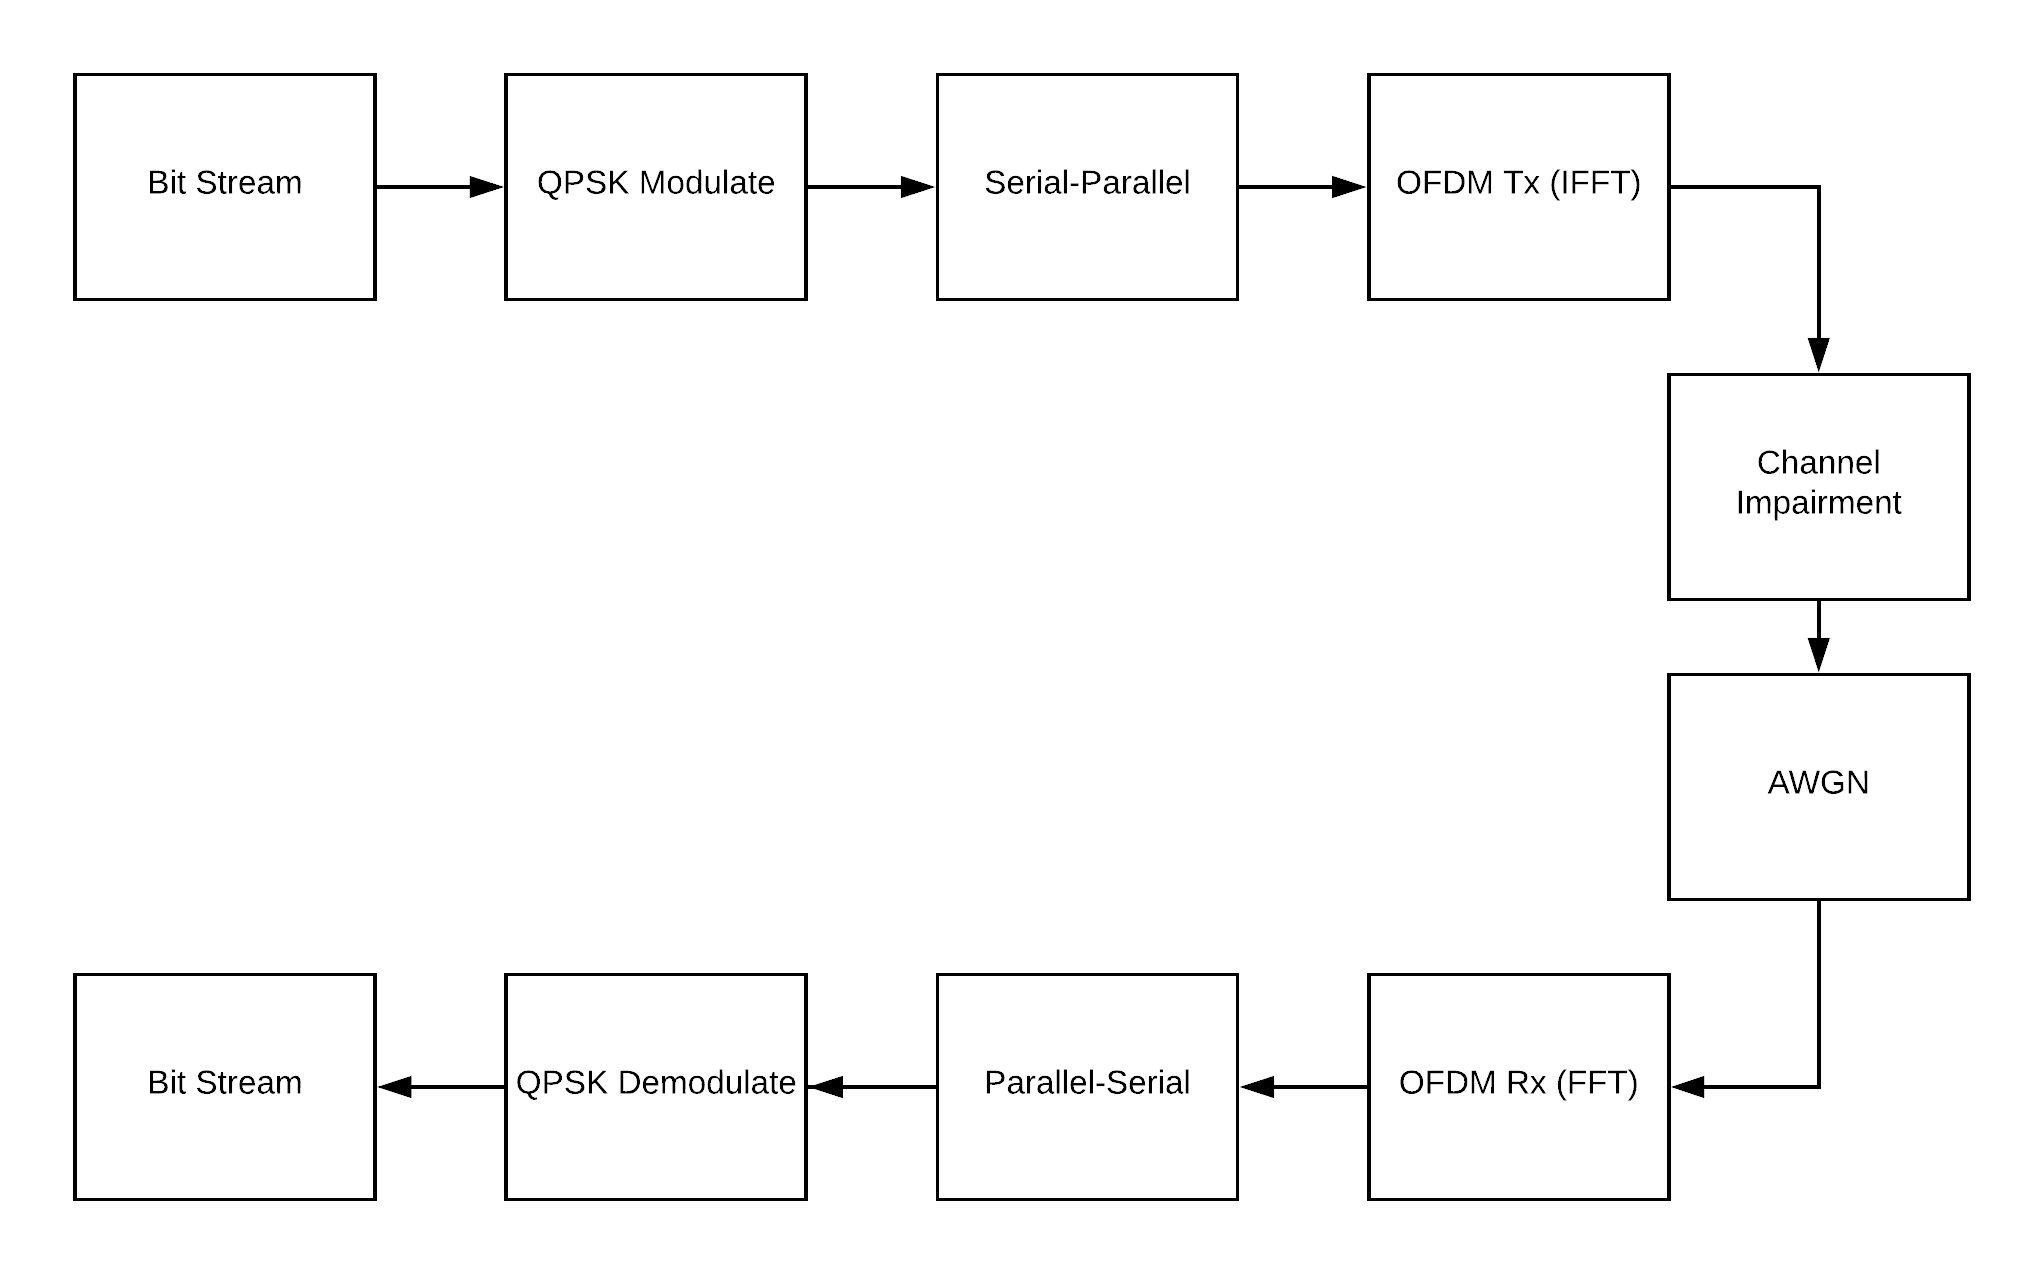
\includegraphics[width=\textwidth]{./%
	Figures/System/SystemModel.png}
	\caption{System Model}
	\label{fig:SysModel}
\end{figure}
Figure \ref{fig:SysModel} depicts the general %
outline of the system model that has been %
developed. This section will focus on %
developing all the components that will %
be common to all the later sections as %
well as section specific components.
\FloatBarrier
The primary aim of the time invariant %
model was to establish the convergence %
of the LMS algorithm with an OFDM %
transmission scheme, equalising in the %
\emph{frequency} domain.
\begin{figure}[ht]
	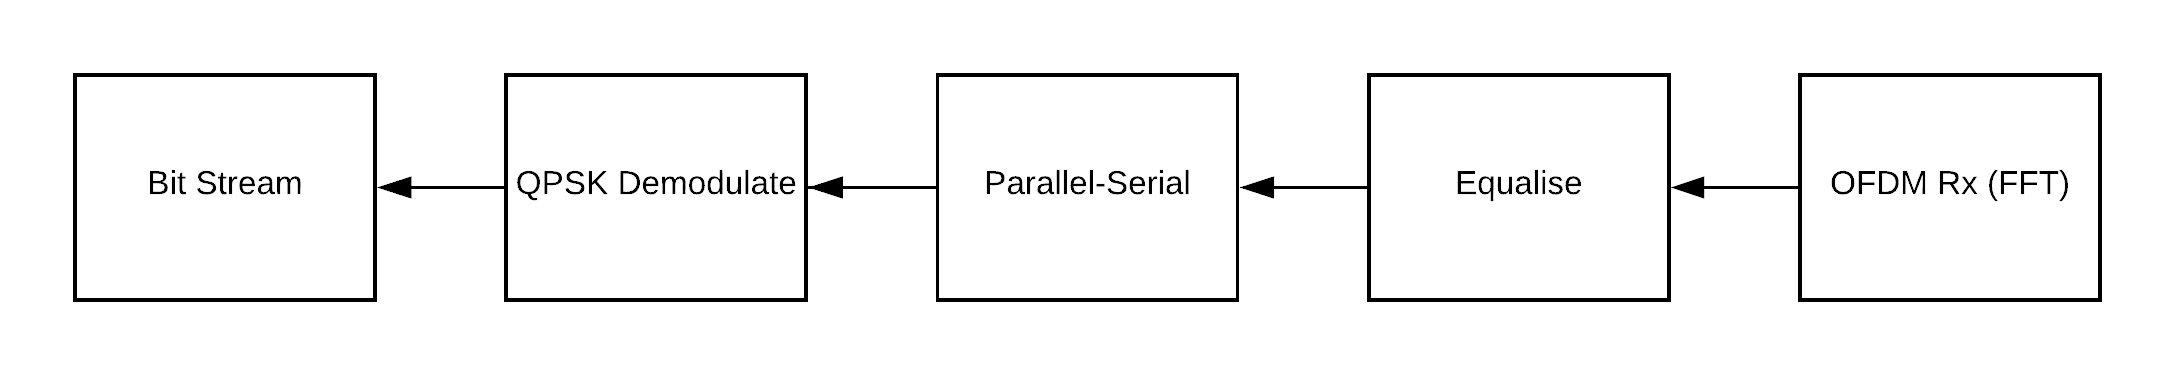
\includegraphics[width=\textwidth]{./%
	Figures/System/RxEqualisation.png}
	\caption{Added equalisation step}
	\label{fig:RxEqualiser}
\end{figure}
Figure \ref{fig:RxEqualiser} illustrates %
the location of the equaliser in this model, %
immediately after the FFT and before the %
parallel to serial step. By designing %
the OFDM subcarrier bandwidth to be %
significantly less than the coherence %
bandwidth of the fading channel, a simple %
version of the LMS filter with only one %
filter coefficient can be assigned to %
each subcarrier for equalisation as %
illustrated in figure \ref{fig:Frequency%
LMS}.
\FloatBarrier
\begin{figure}[ht]
	\centering
	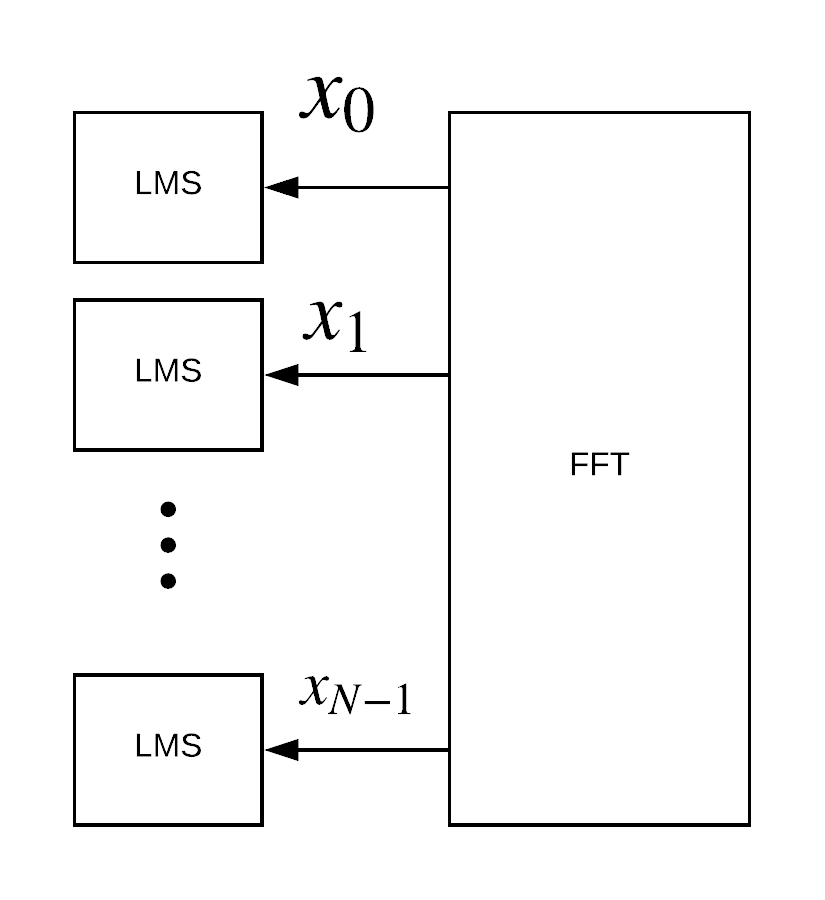
\includegraphics[width=0.5\textwidth]{./%
	Figures/System/FrequencyDomainLMS.png}
	\caption{Single Tap LMS on each Sub%
	carrier}
	\label{fig:FrequencyLMS}
\end{figure}
\FloatBarrier
\subsection{Bit Stream}
The bit stream needs to be selected to model %
a believable source of data. It can be shown %
that without further information, data %
in digital communications systems can be %
modeled as a Bernoulli distribution. %TODO: Cite this
My model simulates this using MATLAB's in-built %
\texttt{randi} function which generates %
a random vector $\vec{X}$ where each %
random variable $X$ can take on values from %
a user defined set of integers and is %
uniformly distributed, i.e. where each integer %
has an equally likely chance of occuring. In %
the special case of the Bernoulli distribution %
the set of integers can be defined as $\{0,1\}$.

\subsection{QPSK Modulation and Demodulation}
\FloatBarrier
QPSK or Quadrature Phase Shift Keying is a popular %
modulation scheme. I've chosen to use it primarily %
for its simplicity but also because it contains both
an in-phase and a quadrature component, which are %
the elements required to construct %
Quadrature Amplitude Modulation (QAM) %
which is the current modulation scheme employed %
in 4G systems % TODO: Find a citation for this.
and are seriously being considered for 5G systems.
\begin{figure}[ht]
	\centering
	\includegraphics[width=0.7\textwidth]{./%
	Figures/System/QPSKScatterplotWithA%
	WGN.png}
	\caption{QPSK Constellation, red stars %
	indicate constellation points, blue %
	points are due to noise}
	\label{fig:QPSKConstellation}
\end{figure}

Figure \ref{fig:QPSKConstellation} shows what %
a QPSK constellation looks like and how a %
received signal might appear when AWGN has %
been added to it. To normalise that average %
symbol energy to 1 the constellation points %
are defined at $\{\frac{\sqrt{2}}{2} + \frac{%
\sqrt{2}}{2}i, \frac{\sqrt{2}}{2} - %
\frac{\sqrt{2}}{2}i, -\frac{\sqrt{2}%
}{2} + \frac{\sqrt{2}}{2}i, %
-\frac{\sqrt{2}}{2} - \frac{\sqrt{2}%
}{2}i\}$ such that when the average %
energy is evaluated
\begin{align}
	E\left[E_s\right] = \frac{1}{4} \sum_{k=1}^{4} %
	\lvert E_{s_{k}} \rvert = 1
\end{align}
where $E_{s_{k}}$ is the symbol energy of the the %
$k\text{th}$ element in the symbol set. A QPSK %
modulation scheme has a symbol set of size $4$. %
So is capable of transmitting $log_{2}(4)$ bits %
per symbol. In general a M-QAM modulation scheme %
is able to transmit $log_{2}(M)$ bits per symbol. %
A grey mapping between pairs of bits to the QPSK %
constellation needs to be chosen so that symbol %
errors that are due to the received symbol mapping %
incorrectly to a neighbouring symbol than what was %
desired will introduce only one bit error instead %
of multiple, it can be shown that grey mapping %
minimises the bit error rate caused by %
symbol errors. %TODO: Find a citation for grey mapping

MATLAB's Communications System Toolbox offers %
a system object name \texttt{comm.QPSKModulator} which %
will perform the grey mapping of pairs of bits in a %
bit stream to QPSK constellation points and perform %
the energy normalisation.

Paired with the \texttt{comm.QPSKModulator} MATLAB also %
provides a \texttt{comm.QPSKDemodulator} which performs %
performs maximum likelihood detection and maps %
the received QPSK constellation back to a bit %
stream.

\subsection{OFDM}

OFDM has been covered in some detail in chapter %
\ref{chap:OFDM} so here I'll focus on the simulation %
implementation. MATLAB's communication systems %
toolbox provides an \texttt{comm.OFDMModulator} which %
takes in an input stream of symbols and performs %
an IFFT followed by an IFFT shift to place the DC %
components in the centre. It also prepends the %
last $\mu$ samples of the output of the IFFT to %
generate a cyclic prefix and allows the use %
of a DC Null, the DC null will be relevant in %
our discussion on the USRP model.

\subsection{AWGN}

The power of additive white gaussian noise $\sigma_n^{2}$ %
was defined relative to the transmit signal power, through %
the following evaluation

\texttt{%
powerdB = 10*log10(var(OFDM\_Symbol));\\%
snr = EbNo + 10*log10(BitsPerSymbol);\\%
noiseVar = 10\textasciicircum(0.1*(powerdB-snr));}

here \texttt{var(OFDM\_Symbol)} is being evaluated %
as 
\begin{align}
	\frac{1}{N} %
	\sum_{n=0}^{N-1} \lvert\lvert \texttt{OFDM\_Symbol}%
	(n) \rvert\rvert^{2}
\end{align}

Where $N$ is the length of the FFT. \texttt{EbNo} is a %
variable which defines the normalised bit energy %
to noise power spectral density and is % TODO: Cite EbNo
expressed as
\begin{align}
	\frac{E_b}{N_0} = \frac{S}{R_b} \div 
	\frac{\sigma_n^{2}}{B}
\end{align}
where $S$ is the average received signal power, %
$R_b$ is the bit rate, $\sigma_n^{2}$ is the %
total additive white gaussian noise power and %
$B$ is the total signal bandwidth. The relation %
between SNR and $E_b/N_0$ is as follows
\begin{align}
	\frac{S}{\sigma_n^{2}} = \frac{E_b}{N_0}
	\frac{R_b}{B}
\end{align}
A modulation scheme such as QPSK doubles the bit %
rate relative to a binary scheme such as on off %
keying or binary phase shift keying (BPSK), so %
SNR needs to be multipled by $2$ for the different %
schemes to experience the same normalised %
signal to noise ratio, given the same signal bandwidth. %
In log units multiplication %
is evaluated as addition as can be seen above.

MATLAB's Commmunications System Toolbox system object %
\texttt{comm.AWGNChannel} takes an input stream of %
symbols and generates complex gaussian noise with %
zero mean and defined variance. This noise is then %
summed with the samples in the stream to make a noisy %
received signal. In the case of the system model shown in %
figure \ref{fig:SysModel}, the power of the complex %
additive white gaussian noise calculated based on the transmit %
power before channel impairments. This is because the Rayleigh %
fading channel impairment does not affect all subbands equally as %
it is a frequency selective effect, so setting the noise power based %
on the post channel impairment signal would disproportinately affect %
the subcarriers that are experiencing deep fades.

\subsection{Channel Impairment}
\label{sec:TIChannelImpairment}
The channel impairment designed for the time invariant model %
will be different to the channel impairment designed for the time varying model. %
Here the channel impairment will be chosen as a random complex gaussian that %
defines the fading in the frequency domain. For the purpose of testing the convergence %
of the LMS algorithm, a flat fading scenario is introduced where each subcarrier %
is multiplied by the same coefficient $w$ as illustrated in figure \ref{fig:TIChannel}.
\begin{figure}[ht]
	\includegraphics[width=\textwidth]{./Figures/System/%
	ChannelTimeInvariant.png}
	\caption{Time Invariant Flat Fading Channel Model}
	\label{fig:TIChannel}
\end{figure}
By introducing AWGN to the system after channel impairment and then %
applying the LMS individually to each subcarrier in the frequency domain, %
ensemble averages can be taken for differing channel conditions simply by %
increasing the number of subcarriers. A subcarrier count of $1024$ was %
chosen to generate the time invariant results discussed in the next chapter. %

\subsection{Equalisation}
\label{subsec:Equalisation}
As illustrated in figure \ref{fig:FrequencyLMS}, a frequency domain %
LMS scheme was made with a single tap variant of the LMS algorithm on %
each subcarrier. As discussed in previous chapters, this can be done %
because the subcarrier bandwidths have been designed to be significantly %
narrower than the coherence bandwidth, so can be approximated with a %
single filter coefficient. This approximation has been made explicit in this %
time invariant model as described in section \ref{sec:TIChannelImpairment}. %

The single tap LMS approximation follows closely from the development of the %
LMS filter in section \ref{sec:LMS}, in particular we take equation \ref{eq:SimplifiedLMSUpdate} %
and replace the vector of coefficients $\hat{\bold{w}}(n+1)$ and $\hat{\bold{w}}(n)$ with scalar %
versions, and the vector of filter inputs $\bold{u}(n)$ with a scalar input. Giving the %
new expression
\begin{align}
	\hat{w}(n+1) = \hat{w}(n) + \mu u(n) e^{*}(n)
	\label{eq:ScalarLMS}
\end{align}
This version of the LMS update is the computationally simplest %
the LMS can be with two multiplications and one addition. %
The constant computational complexity of the designed LMS means %
that the complexity of this filtering scheme grows with the %
the size of the FFT needed to ensure that the subcarrier bandwidth %
is narrower than the coherence frequency of the fading channel, and %
has computational complexity $\mathcal{O}(N log(N))$. This scalar version %
of the LMS filter is substituted into the LMS blocks shown in figure %
\ref{fig:FrequencyLMS} at the receiver.

In a similar fashion the NLMS filter can be developed with a scalar equation %
\begin{align}
	\hat{w}(n+1) = \hat{w}(n) + \frac{\mu}{\lvert u(n) \rvert^{2}} %
	u(n) e^{*}(n)
	\label{eq:ScalarNLMS}
\end{align}
and substitued into the LMS blocks in figure \ref{fig:FrequencyLMS} to %
evaluate the performance of the NLMS filter.

\section{Time Varying System Model}

The time varying system model only contains two key differences to the %
time invariant model. The first is the introduction of the time-varying Rayleigh %
and Rician channel models, these channel models have been simulated using %
the filtered white gaussian noise method. The Rayleigh and Rician fading %
channels introduce design constraints to the model not present in the %
simplified time invariant model examined in section %
\ref{sec:TIModel} regarding subcarrier bandwidth and coherence %
frequency as well as the OFDM symbol time and channel %
coherence time. The second key difference is the introduction %
of a decision directed scheme for the LMS %
filter to examine its tracking performance after achieving %
the optimal Wiener solution.

\subsection{Filtered White Gaussian Noise Channel Simulation}

The time varying fading channel can be broken down into three %
steps. The power delay definition needs to be defined, using the %
power delay profile the average powers of each multipath %
coefficient can be defined. Once this is done the time varying %
component of the fading channel needs to be introduced, %
the method of choice for this simulation will be one of filtered %
white gaussian noise. 
\subsubsection{The Power Delay Profile}

The power delay profile is critical in scaling the average power %
of each multipath coefficient. In figure \ref{fig:ChannelFilterSimulation} %
an illustration of the simulation mechanism by which a single channel %
coefficient process can be generated, $\sigma_{n}$ represents %
the scaling factor to ensure that the $n\text{th}$ coefficient %
of the multipath channel $h(\tau_{n};t)$ has average power %
$\sigma_{n}^{2}$. In the simplest form of an uncorrelated %
tap-gain model \cite{Jer00} 
\begin{align}
	E\left[\lvert h(\tau_{n};t) \rvert^{2} \right] = %
	\sigma_{n}^{2} = T^{2}p(nT)
	\label{eq:TapPower}
\end{align}
where $p(nT)$ is the sampled version of a diffuse power %
delay profile where $T$ is the sampling period. Or of a %
discrete multipath channel where the multipath coefficients %
are symbol spaced. For the purpose of my investigation I %
will not consider the case of a discrete multipath channel %
where the multipath channel coefficients are not symbol %
spaced since in general this requires us to filter the power %
delay profile by the measurement bandlimiting filter (i.e., matched filtering) %
and so more information would be needed about the pulse shaping %
used. With symbol spacing an assumption is made that the filters used %
are nyquist in nature and so there are no additional components %
introduced by neighbouring multipath coefficients.

\subsubsection{Filtered White Gaussian Noise}

In chapter \ref{chap:ChannelModeling} the time-varying nature of %
the fading channel was established as being closely related to the %
doppler shift of the signal and the maximum doppler frequency $f_d$. %
The doppler spectrum chosen for simulation is the Jakes spectrum as %
defined in equation \ref{eq:JakesSpectrum} as it is a popular spectrum %
widely used in the literature. %TODO: Cite the literature

The filtered white gaussian noise approach aims to recreate this %
time varying effect by directly filtering the random noise representing %
the scattering with a doppler spectrum in the frequency domain\cite{%
MIMO-OFDM10, Iskander}. 
\begin{figure}[ht]
	\includegraphics[width=\textwidth]{./Figures/System/%
	FilteringProcess.png}
	\caption{Channel Filter Tap Generation}
	\label{fig:ChannelFilterSimulation}
\end{figure}
Figure \ref{fig:ChannelFilterSimulation} illustrates the process %
used to generate each individual coefficient in the discrete %
multipath channel. $z(t)$ is an independent and identically %
distributed (i.i.d) time series where at each timestep $t$, % 
$z(t)\sim\mathcal{N}(0,1)$ (is normally distributed %
with mean $0$ and standard deviation $1$), $S(\nu)$ is the %
Jakes doppler spectrum as described in equation %
\ref{eq:JakesSpectrum} and $\sigma_n$ is %
a scaling factor to ensure the average power of the coefficient %
matches that of the power delay profile.

MATLAB's Communications System Toolbox provides a system object %
\texttt{comm.RayleighChannel}, which implements the filtered %
white gaussian noise method of simulation as described in 
\cite{Iskander}. Rician distributions are implemented slightly %
differently where the Rician coefficients are further scaled by a %
deterministic component with a specular to %
scattered power ratio $K$ as described in equation %
\ref{eq:KFactor}. The Rician fading component is scaled by %
\begin{align}
	h(\tau;t) = \sigma_n\left[ \frac{z_{k}\left[n\right]}
	{\sqrt{K + 1}} + 
	\sqrt{\frac{K}{K+1}}\right]
\end{align}
Where $z_{k}$ is the filtered noise output of the doppler filter 
\cite{Iskander} immediately after the normalization step in figure %
\ref{fig:ChannelFilterSimulation}.

\subsection{Decision Directed Performance}

It's important to evaluate the performance of the time varying model %
in a decision directed scheme. That is, after a given %
training period the Wiener solution has been found using an adaptive %
filtering approach. In particular it is of interest how long the %
adaptive filtering approach can maintain a solution that is near %
optimal without additional further training %
information. A decision directed model is one where the %
output of the equaliser is fed into the maximum likelihood %
decision slicer, and the output of the decision slicer is fed back %
into the equaliser as the desired %
output in the update equation (\ref{eq:ScalarLMS} and \ref{eq:%
ScalarNLMS}), where $e(n) = d(n) - y(n)$ as illustrated in figure %
\ref{fig:DDLMS}.
\begin{figure}[ht]
	\includegraphics[width=\textwidth]{./Figures/System/%
	DecisionDirectedOperation.png}
	\caption{LMS in Decision Directed Operation}
	\label{fig:DDLMS}
\end{figure}
This region of operation introduces some delay to the system as %
the decision slicer needs to map the received symbol onto the %
nearest constellation point before the adaptive step can begin. %
As discussed in section \ref{sec:TIModel} the decision slicer %
being used here is MATLAB's \texttt{comm.QPSKDemodulator} %
from the Communications System Toolbox.

\section{USRP Implementation of the Time Varying System Model}

Figure \ref{fig:USRPDiagram} shows the hardware diagram %
for the radio front-end of the national instruments %
software defined radio. The radio front end uses a homodyne %
receiver architecture over a more traditional heterodyne %
architecture as shown in the DUC (Direct Up Conversion) and %
DDC (Direct Down Conversion) blocks in the diagram. The homodyne %
receiver architecture offers a simpler hardware receiver design %
which is in line with the software defined radio philosophy of %
moving the signal processing to software.
\begin{figure}[ht]
	\includegraphics[width=\textwidth]{./Figures/System/%
	USRP2943R.png}
	\caption{System Diagram for the Software Defined Radio%
	\cite{USRPDiagram}}
	\label{fig:USRPDiagram}
\end{figure}

\subsection{Direct Conversion Architecture}
\label{subsec:DirectConversion}
The direct conversion or homodyne architecture converts received %
bandpass signals directly to baseband signals without the need for %
an intermediate frequency. This is done by selecting a local %
oscillator (LO) frequency to be the same as the centre %
frequency of the bandpass signal.
\begin{figure}[ht]
	\centering
	\includegraphics[width=\textwidth]{./Figures/System/%
	DirectConversionScheme.png}
	\caption{Direct Down Conversion Process}
	\label{fig:DDC}
\end{figure}
Figure \ref{fig:DDC} illustrates this process where $I(t)$ is the %
in phase component and $Q(t)$ is the quadrature component. %
Although the direct conversion process offers advantages to the %
heterodyne architecture in terms of hardware simplicity, it comes %
with a key disadvantage in that if any part of the LO signal %
leaks into the RF input stream it introduces distortion into the %
received baseband signal as a DC offset. OFDM avoids %
additional interference caused by this LO leakage by inserting %
null carriers in and around the DC component.

\subsection{Transmitter Model}

The radio transmitter model was modeled on the finite %
synchronous transmit example model given in the LabView %
Instrument IO library. A diagram of transmitter is given %
in appendix \ref{app:TxSysModel}. %
The synchronous finite capture allows me to %
transmit and receive simultaneously, triggered on %
an internal clock, this removes the problem of %
synchronisation that would trouble a real %
wireless communication system and lets us %
constrain our attention to purely the effectiveness %
of the adaptive filtering algorithm at the receiver. %

In addition to the use of the synchronous transmit and %
receive an upsampling factor of $4$ has been used %
to ensure that the samples definitely occur on the %
modulated amplitude levels and not on any edges that %
occur to compensate for any fractional delay that %
might be present.


\subsection{Receiver Model}
\FloatBarrier
The radio receiver model was modeled on the finite %
synchronous receiver example model given in the Lab%
View Instrument IO library. A diagram of the receiver %
is given in appendix \ref{app:RxSysModel}. %

Unequalised the receiver constellation is a ring as is %
illustrated in figure \ref{fig:ReceivedRing}. The line %
leading from the centre of the ring to the edge is %
caused by the null carriers and the DC offset distortion %
caused by the LO as discussed in section \ref{subsec:Direct%
Conversion}. The ring itself is caused by the frequency offset %
between the LO that shifts the bandpass signal to the baseband %
and the central frequencies of each of the subcarriers. This %
frequency offset effect causes a rotation from the constellation %
point equal to the difference between the LO frequency and the %
central frequency of the subcarrier as described by 
\begin{align}
	r(t) = r'(t)e^{j 2\pi f_{e}t}
\end{align}
where $r'(t)$ is the ideal received constellation $r(t)$ is %
the received constellation and $f_{e}$ is the difference %
between the LO frequency and the subcarrier frequency.
\begin{figure}[ht]
	\centering
	\includegraphics[width=0.6\textwidth]{./Figures/System/%
	UnequalisedRing.png}
	\caption{Received Constellation before equalisation}
	\label{fig:ReceivedRing}
\end{figure}
\FloatBarrier
\subsection{Equalisation and Top Level Design}
The equalisation step in the USRP model follows %
the diagram in figure \ref{fig:USRPEqualisation}. The transmitted %
symbols are passed to the equalisation block and the received %
symbols are also passed to the equalisation block. Within this block %
the LMS, NLMS and zero forcing equalisers are implemented as %
described in chapter \ref{chap:AdaptiveFiltering} and %
\ref{subsec:Equalisation}.
\begin{figure}[ht]
	\centering
	\includegraphics[width=0.6\textwidth]{./Figures/System/%
	USRPEqualisation.png}
	\caption{USRP Equalisation}
	\label{fig:USRPEqualisation}
\end{figure}
\subsection{AWGN}
\subsection{Multipath Channel Simulation}

\chapter{Results}
\label{chap:Results}
\section{Time Invariant Simulation Results}
In this section I will be covering my results for the time-invariant %
model as described in chapter \ref{chap:System}. The results will be %
broken down into two sections, first we will examine the %
LMS algorithm and its convergence, then we will examine the NLMS %
algorithm.

\subsection{Least Mean Square}
\FloatBarrier
The three key measures of the LMS algorithm are it is mean square %
error, mean square deviation, and excess mean square error. %
The mean square error is a measure of how close the estimate %
is to the desired output and is defined as 
\begin{align}
	J = E\left[ \lvert d(n) - y(n) \rvert^{2} \right]
\end{align}
Mean square deviation is a measure of how much error there is %
between the optimal filter coefficients and the estimated %
channel coefficients and is defined as
\begin{align}
	\mathscr{D} = E\left[ \lvert w_{o}(n) - \hat{w}(n) \rvert^{2} \right]
\end{align}
And the excess mean square error is a measure of how much %
difference there is between the mean square error of the %
optimal solution and the estimated solution and is defined as
\begin{align}
	J_{\text{excess}} = J_{o} - J
\end{align}
Figures \ref{fig:LMS-MSE}, \ref{fig:LMS-MSD}, and \ref{fig:LMS-EMSE} %
show the results for mean square error, mean square deviation and %
excess mean square error for the LMS filter under a variety of %
different step sizes $\mu$.

\begin{figure}[ht]
	\centering
	\begin{minipage}{0.49\textwidth}
		\centering
		\includegraphics[width=\linewidth]{./Figures/Results/%
		TimeInvariantLMS/NoDivergence/%
		ExcessMeanSquareError.png}
		\captionsetup{width=0.75\linewidth}
		\caption{Excess Mean Square Error of LMS}
		\label{fig:LMS-EMSE}
	\end{minipage}
	\begin{minipage}{0.49\textwidth}
		\centering
		\includegraphics[width=\linewidth]{./Figures/Results/%
		TimeInvariantLMS/NoDivergence/MeanSquareDeviation.png}
		\captionsetup{width=0.75\linewidth}
		\caption{Mean Square Deviation of LMS}
		\label{fig:LMS-MSD}
	\end{minipage}
\end{figure}
\begin{figure}[ht]
	\centering
	\includegraphics[width=0.55\textwidth]{./Figures/Results/%
	TimeInvariantLMS/NoDivergence/MeanSquareError.png}
	\captionsetup{width=0.75\linewidth}
	\caption{Mean Square Error of LMS}
	\label{fig:LMS-MSE}
\end{figure}

It is apparent for the figures that as the step size increases the %
rate of convergence increases as well. Recalling the discussion in %
chapter \ref{chap:AdaptiveFiltering} on adaptive filtering, this %
agrees with the intuition of larger step sizes moving more quickly %
down the error surface towards the optimum solution. % 
Drawing our attention to figure \ref{fig:LMS-EMSE} it is clear that %
for larger step sizes the excess mean square error is higher %
in steady state. This is also in agreement with with the stochastic %
gradient theory\cite{Hay02}. When the step size is large, noise %
will cause the LMS filter to overshoot the optimum solution %
and oscillate around it, leading to larger excess mean square %
error or misadjustment. This confirms that given the time invariant %
system model the LMS filter operating in the frequency domain does %
in fact converge to the optimal solution and that %
the expected tradeoff between convergence time and misadjustment is %
present.
\begin{figure}[ht]
	\centering
	\begin{minipage}{0.49\textwidth}
		\includegraphics[width=\linewidth]{./Figures/Results/%
		TimeInvariantLMS/Divergence/MeanSquareDeviation.png}
		\captionsetup{width=0.75\linewidth}
		\caption{Mean Square Deviation diverging of LMS}
		\label{fig:LMS-MSD-Diverge}
	\end{minipage}
	\begin{minipage}{0.49\textwidth}
		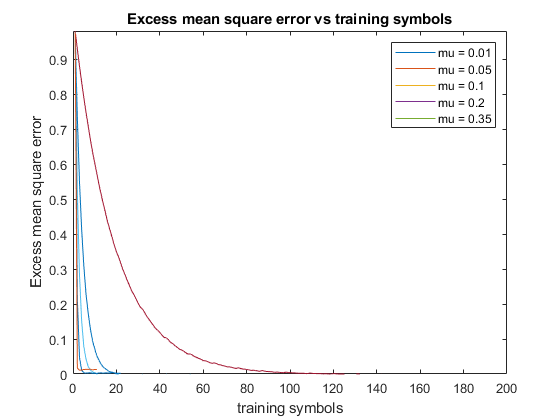
\includegraphics[width=\linewidth]{./Figures/Results/%
		TimeInvariantLMS/Divergence/ExcessMeanSquareError.png}
		\captionsetup{width=0.75\linewidth}
		\caption{Excess Mean Square Error diverging of LMS}
		\label{fig:LMS-EMSE-Diverge}
	\end{minipage}
\end{figure}
\begin{figure}[ht]
	\centering
	\includegraphics[width=0.55\textwidth]{./Figures/Results/%
	TimeInvariantLMS/Divergence/MeanSquareError.png}
	\captionsetup{width=0.75\linewidth}
	\caption{Mean Square Error diverging of LMS}
	\label{fig:LMS-MSE-Diverge}
\end{figure}
Table \ref{tab:LMS} lists that valid step sizes for $\mu$ range %
between $0$ and $2/(M S_{\text{max}})$, however %
this is only valid for when $M$ is large. Instead we will %
examine the divergence of the LMS filter under the %
condition that $\mu$ must be between:
\begin{align}
	0 < \mu < \frac{2}{\sigma^{2}}
	\label{eq:LMS-Stability}
\end{align}
Where $\sigma^{2}$ is the variance in the input signal, and can also %
be thought of as the average power of the input signal. This follows %
directly from the conditions imposed upon step size by the gradient %
descent optimisation method shown below \cite{Hay02}.
\begin{align}
	0 < \mu < \frac{2}{\lambda}
\end{align}
Figures \ref{fig:LMS-MSE-Diverge}, %
\ref{fig:LMS-MSD-Diverge}, \ref{fig:LMS-EMSE-Diverge} are %
show systems that diverge at a $\mu = 0.35$. This occurs %
when the randomly generated fading is very large and reduces %
the upper bound in equation \ref{eq:LMS-Stability} to beneath %
$\mu$.
\FloatBarrier
\subsection{Normalized Least Mean Square}
\FloatBarrier
Similarly to the LMS filter, the NLMS filter also demonstrates %
convergence to the optimal solution as can be %
seen in figures \ref{fig:NLMS-MSE}, \ref{fig:NLMS-MSD}, %
and \ref{fig:NLMS-EMSE}. It's very apparent when %
comparing the $\mu = 0.05$ lines of the LMS and NLMS filters %
that the NLMS filter has faster convergence. The NLMS filter %
also has a greater range of convergent choices for %
$\mu$ as can be seen from the legend. This is in agreement %
with equation \ref{eq:SayedNLMSBound}. At higher choices of %
$\mu$ the NLMS also has a much higher misadjustment as can be %
seen in figure \ref{fig:NLMS-EMSE} which is a result of the %
faster rate of convergence. The regularisation parameter chosen %
for this NLMS experiment is chosen to be $0.05$.

\begin{figure}[ht]
	\centering
	\begin{minipage}{0.49\textwidth}
		\includegraphics[width=\linewidth]{./Figures/Results/%
		TimeInvariantNLMS/NoDivergence/%
		MeanSquareDeviation.png}
		\captionsetup{width=0.75\linewidth}
		\caption{Mean Square Deviation of NLMS}
		\label{fig:NLMS-MSD}
	\end{minipage}
	\begin{minipage}{0.49\textwidth}
		\includegraphics[width=\linewidth]{./Figures/Results/%
		TimeInvariantNLMS/NoDivergence/%
		ExcessMeanSquareError.png}
		\captionsetup{width=0.75\linewidth}
		\caption{Excess Mean Square Deviation of NLMS}
		\label{fig:NLMS-EMSE}
	\end{minipage}
\end{figure}
\begin{figure}[ht]
	\centering
	\includegraphics[width=0.55\textwidth]{./Figures/Results/%
	TimeInvariantNLMS/NoDivergence/MeanSquareError.png}
	\captionsetup{width=0.75\linewidth}
	\caption{Mean Square Error of NLMS}
	\label{fig:NLMS-MSE}
\end{figure}

In figures \ref{fig:NLMS-MSE-Diverge}, \ref{fig:NLMS-MSD-Diverge}, %
and \ref{fig:NLMS-EMSE-Diverge} it is apparent that %
for choices of $\mu$ greater than $2$ the NLMS algorithm diverges.
\begin{figure}[ht]
	\centering
	\begin{minipage}{0.49\textwidth}
		\centering
		\includegraphics[width=\linewidth]{./Figures/Results/%
		TimeInvariantNLMS/Divergence/MeanSquareDeviation.png}
		\captionsetup{width=0.75\linewidth}
		\caption{Mean Square Deviation Divergence of NLMS}
		\label{fig:NLMS-MSD-Diverge}
	\end{minipage}
	\begin{minipage}{0.49\textwidth}
		\centering
		\includegraphics[width=\linewidth]{./Figures/Results/%
		TimeInvariantNLMS/Divergence/%
		ExcessMeanSquareError.png}
		\captionsetup{width=0.75\linewidth}
		\caption{Excess Mean Square Error Divergence of NLMS}
		\label{fig:NLMS-EMSE-Diverge}
	\end{minipage}
\end{figure}
\begin{figure}[ht]
	\centering
	\includegraphics[width=0.55\textwidth]{./Figures/Results/%
	TimeInvariantNLMS/Divergence/MeanSquareError.png}
	\captionsetup{width=0.75\linewidth}
	\caption{Mean Square Error Divergence of NLMS}
	\label{fig:NLMS-MSE-Diverge}
\end{figure}

\section{Time Varying Simulation Results}
\label{sec:TVResults}
The time varying MATLAB simulation results covered in this section %
vary four different parameters, coherence time, SNR, decision %
direction and cyclic prefix length. Coherence time is varied as %
0.17, 1.7 and 17 seconds. $E_b/N_0$ is varied as $12\text{dB}$ and %
$30\text{dB}$. Decision direction is simply varied as either %
being decision directed or not decision directed, and the cyclic %
prefix length is varied as 10 samples and 56 samples. The Wiener %
solution evaluated throughout this section is an approximation %
of the Wiener solution as the time-varying nature of the problem %
means that the distortion is no longer ergodic and evaluating the %
expectations in equations \ref{eq:WienerAutocorrelation} and %
\ref{eq:WienerCrossCorrelation} can no longer be found by %
averaging in time. The Wiener solution approximation is made %
by constraining the window length for averaging the %
autocorrelation function to one order of magnitude smaller %
than the coherence time (i.e., when the coherence time is 17 %
seconds, the averaging window for evaluating the wiener solution %
will be on the order of 1 second).
\begin{figure}[ht]
	\centering
	\begin{minipage}{0.49\textwidth}
		\centering
		\includegraphics[width=\linewidth]{./Figures%
		/Results/%
	LMS_Time_Varying/LongCP/DD/HighSNR/LongTimeCoherence/%
	MeanSquareError.png}
		\captionsetup{width=0.75\linewidth}
		\caption{Mean Square Error of Time Varying LMS with 
		a long cyclic prefix, in decision directed operation,
		with a long coherence time at high SNR}
	\end{minipage}
	\begin{minipage}{0.49\textwidth}
		\centering
		\includegraphics[width=\linewidth]{./Figures/Results/%
	NLMS_Time_Varying/LongCP/DD/HighSNR/LongTimeCoherence/%
	MeanSquareError.png}
		\captionsetup{width=0.75\linewidth}
		\caption{Mean Square Error of Time Varying NLMS with 
		a long cyclic prefix, in decision directed operation,
		with a long coherence time at high SNR}
	\end{minipage}
\end{figure}
\begin{figure}[ht]
	\centering
	\begin{minipage}{0.49\textwidth}
		\centering
		\includegraphics[width=\linewidth]{./Figures/Results/%
	LMS_Time_Varying/LongCP/DD/HighSNR/MediumTimeCoherence/%
	MeanSquareError.png}
		\captionsetup{width=0.75\linewidth}
		\caption{Mean square error of time varying LMS with a 
		long cyclic prefix, in decision directed operation, 
		with a medium coherence time at high SNR}
		\label{fig:Medium-High-Directed-Long}
	\end{minipage}
	\begin{minipage}{0.49\textwidth}
		\centering
		\includegraphics[width=\linewidth]{./Figures/Results/%
	NLMS_Time_Varying/LongCP/DD/HighSNR/MediumTimeCoherence/%
	MeanSquareError.png}
		\captionsetup{width=0.75\linewidth}
		\caption{Mean square error of time varying NLMS with 
		a long cyclic prefix, in decision directed operation, 
		with a medium coherence time at high SNR}
	\end{minipage}
\end{figure}

\begin{figure}[ht]
	\centering
	\begin{minipage}{0.49\textwidth}
		\centering
		\includegraphics[width=\linewidth]{./Figures/Results/%
	LMS_Time_Varying/LongCP/DD/HighSNR/ShortTimeCoherence/%
	MeanSquareError.png}
		\captionsetup{width=0.75\linewidth}
		\caption{Mean square error of time varying LMS with a 
		long cyclic prefix, in decision directed operation,
		with a short coherence time at high SNR}
	\end{minipage}
	\begin{minipage}{0.49\textwidth}
		\centering
		\includegraphics[width=\linewidth]{./Figures/Results/%
	NLMS_Time_Varying/LongCP/DD/HighSNR/ShortTimeCoherence/%
	MeanSquareError.png}
		\captionsetup{width=0.75\linewidth}
		\caption{Mean square error of time varying NLMS with 
		a long cyclic prefix, in decision directed operation,
		with a short coherence time at high SNR}
		\label{fig:NLMS-Short-High-Directed-Long}
	\end{minipage}
\end{figure}

\begin{figure}[ht]
	\begin{minipage}{0.49\textwidth}
		\includegraphics[width=\linewidth]{./Figures/Results/%
	LMS_Time_Varying/LongCP/DD/LowSNR/LongTimeCoherence/%
	MeanSquareError.png}
		\captionsetup{width=0.75\linewidth}
		\caption{Mean square error of time varying LMS with a 
		long cyclic prefix, in decision directed operation,
		with a long coherence time at low SNR}
	\end{minipage}
	\begin{minipage}{0.49\textwidth}
		\includegraphics[width=\linewidth]{./Figures/Results/%
	NLMS_Time_Varying/LongCP/DD/LowSNR/LongTimeCoherence/%
	MeanSquareError.png}
		\captionsetup{width=0.75\linewidth}
		\caption{Mean square error of time varying NLMS with 
		a long cyclic prefix, in decision directed operation,
		with a long coherence time at low SNR}
	\end{minipage}
\end{figure}

\begin{figure}[ht]
	\centering
	\begin{minipage}{0.49\textwidth}
		\centering
		\includegraphics[width=\linewidth]{./Figures/Results/%
	LMS_Time_Varying/LongCP/DD/LowSNR/MediumTimeCoherence/%
	MeanSquareError.png}
		\captionsetup{width=0.75\linewidth}
		\caption{Mean square error of time varying LMS with a 
		long cyclic prefix, in decision directed operation, 
		with a medium coherence time at low SNR}
	\end{minipage}
	\begin{minipage}{0.49\textwidth}
		\centering
		\includegraphics[width=\linewidth]{./Figures/Results/%
	NLMS_Time_Varying/LongCP/DD/LowSNR/MediumTimeCoherence/%
	MeanSquareError.png}
		\captionsetup{width=0.75\linewidth}
		\caption{Mean square error of time varying NLMS with 
		a long cyclic prefix, in decision directed operation,
		with a medium coherence time at low SNR}
	\end{minipage}
\end{figure}

\begin{figure}[ht]
	\begin{minipage}{0.49\textwidth}
		\centering
		\includegraphics[width=\linewidth]{./Figures/Results/%
	LMS_Time_Varying/LongCP/DD/LowSNR/ShortTimeCoherence/%
	MeanSquareError.png}
		\captionsetup{width=0.75\linewidth}
		\caption{Mean square error of time varying LMS with a 
		long cyclic prefix, in decision directed operation,
		with a short coherence time at low SNR}
	\end{minipage}
	\begin{minipage}{0.49\textwidth}
		\includegraphics[width=\linewidth]{./Figures/Results/%
	NLMS_Time_Varying/LongCP/DD/LowSNR/ShortTimeCoherence/%
	MeanSquareError.png}
		\captionsetup{width=0.75\linewidth}
		\caption{Mean square error of time varying NLMS with 
		a long cyclic prefix, in decision directed operation,
		with a short coherence time at low SNR}
	\end{minipage}
\end{figure}

\begin{figure}[ht]
	\begin{minipage}{0.49\textwidth}
		\includegraphics[width=\linewidth]{./Figures/Results/%
	LMS_Time_Varying/LongCP/NoDD/HighSNR/LongTimeCoherence/%
	MeanSquareError.png}
		\captionsetup{width=0.75\linewidth}
		\caption{Mean square error of time varying LMS with a 
		long cyclic prefix, with a long coherence time at 
		high SNR}
	\end{minipage}
	\begin{minipage}{0.49\textwidth}
		\includegraphics[width=\linewidth]{./Figures/Results/%
	NLMS_Time_Varying/LongCP/NoDD/HighSNR/LongTimeCoherence/%
	MeanSquareError.png}
		\captionsetup{width=0.75\linewidth}
		\caption{Mean square error of time varying NLMS with 
		a long cyclic prefix, with a long coherence time at 
		high SNR}
	\end{minipage}
\end{figure}

\begin{figure}[ht]
	\begin{minipage}{0.49\textwidth}
		\includegraphics[width=\linewidth]{./Figures/Results/%
	LMS_Time_Varying/LongCP/NoDD/HighSNR/MediumTimeCoherence/%
	MeanSquareError.png}
		\captionsetup{width=0.75\linewidth}
		\caption{Mean square error of time varying LMS with a 
		long cyclic prefix, with a medium coherence time at 
		high SNR}
	\end{minipage}
	\begin{minipage}{0.49\textwidth}
		\includegraphics[width=\linewidth]{./Figures/Results/%
	NLMS_Time_Varying/LongCP/NoDD/HighSNR/MediumTimeCoherence/%
	MeanSquareError.png}
		\captionsetup{width=0.75\linewidth}
		\caption{Mean square error of time varying NLMS with 
		a long cyclic prefix, with a medium coherence time
		at high SNR}
	\end{minipage}
\end{figure}

\begin{figure}[ht]
	\centering
	\begin{minipage}{0.49\textwidth}
		\centering
		\includegraphics[width=\textwidth]{./Figures/Results/%
	LMS_Time_Varying/LongCP/NoDD/HighSNR/ShortTimeCoherence/%
	MeanSquareError.png}
		\captionsetup{width=0.75\linewidth}
		\caption{Mean square error of time varying LMS with a 
		long cyclic prefix, with a short coherence time at 
		high SNR}
		\label{fig:LMS-Short-High-None}
	\end{minipage}
	\begin{minipage}{0.49\textwidth}
		\centering
		\includegraphics[width=\textwidth]{./Figures/Results/%
	NLMS_Time_Varying/LongCP/NoDD/HighSNR/ShortTimeCoherence/%
	MeanSquareError.png}
		\captionsetup{width=0.75\linewidth}
		\caption{Mean square error of time varying NLMS with 
		a long cyclic prefix, with a short coherence time 
		at high SNR}
	\end{minipage}
\end{figure}

\begin{figure}[ht]
	\centering
	\begin{minipage}{0.49\textwidth}
		\centering
		\includegraphics[width=\linewidth]{./Figures/Results/%
	LMS_Time_Varying/LongCP/NoDD/LowSNR/LongTimeCoherence/%
	MeanSquareError.png}
		\captionsetup{width=0.75\linewidth}
		\caption{Mean square error of time varying LMS with a 
		long cyclic prefix, with a long coherence time at 
		low SNR}
	\end{minipage}
	\begin{minipage}{0.49\textwidth}
		\centering
		\includegraphics[width=\linewidth]{./Figures/Results/%
	NLMS_Time_Varying/LongCP/NoDD/LowSNR/LongTimeCoherence/%
	MeanSquareError.png}
		\captionsetup{width=0.75\linewidth}
		\caption{Mean square error of time varying NLMS with 
		a long cyclic prefix, with a long coherence time 
		at low SNR}
		\label{fig:NLMS-Long-Low-None-Long}
	\end{minipage}
\end{figure}

\begin{figure}[ht]
	\centering
	\begin{minipage}{0.49\textwidth}
		\centering
		\includegraphics[width=\linewidth]{./Figures/Results/%
	LMS_Time_Varying/LongCP/NoDD/LowSNR/MediumTimeCoherence/%
	MeanSquareError.png}
		\captionsetup{width=0.75\linewidth}
		\caption{Mean square error of time varying LMS with a 
		long cyclic prefix, with a medium coherence time at 
		low SNR}
	\end{minipage}
	\begin{minipage}{0.49\textwidth}
		\centering
		\includegraphics[width=\linewidth]{./Figures/Results/%
	NLMS_Time_Varying/LongCP/NoDD/LowSNR/MediumTimeCoherence/%
	MeanSquareError.png}
		\captionsetup{width=0.75\linewidth}
		\caption{Mean square error of time varying NLMS with 
		a long cyclic prefix, with a medium coherence time 
		at low SNR}
	\end{minipage}
\end{figure}

\begin{figure}[ht]
	\centering
	\begin{minipage}{0.49\textwidth}
		\centering
		\includegraphics[width=\linewidth]{./Figures/Results/%
	LMS_Time_Varying/LongCP/NoDD/LowSNR/ShortTimeCoherence/%
	MeanSquareError.png}
		\captionsetup{width=0.75\linewidth}
		\caption{Mean square error of time varying LMS with a 
		long cyclic prefix, with a short coherence time at 
		low SNR}
	\end{minipage}
	\begin{minipage}{0.49\textwidth}
		\centering
		\includegraphics[width=\linewidth]{./Figures/Results/%
	NLMS_Time_Varying/LongCP/NoDD/LowSNR/ShortTimeCoherence/%
	MeanSquareError.png}
		\captionsetup{width=0.75\linewidth}
		\caption{Mean square error of time varying NLMS with 
		a long cyclic prefix, with a short coherence time at 
		low SNR}
	\end{minipage}
\end{figure}

\begin{figure}[ht]
	\centering
	\begin{minipage}{0.49\textwidth}
		\centering
		\includegraphics[width=\linewidth]{./Figures/Results/%
	LMS_Time_Varying/ShortCP/DD/HighSNR/LongTimeCoherence/%
	MeanSquareError.png}
		\captionsetup{width=0.75\linewidth}
		\caption{Mean square error of time varying LMS with a 
		short cyclic prefix, in decision directed operation, 
		with a long coherence time at high SNR}
	\end{minipage}
	\begin{minipage}{0.49\textwidth}
		\centering
		\includegraphics[width=\linewidth]{./Figures/Results/%
	NLMS_Time_Varying/ShortCP/DD/HighSNR/LongTimeCoherence/%
	MeanSquareError.png}
		\captionsetup{width=0.75\linewidth}
		\caption{Mean square error of time varying NLMS with 
		a short cyclic prefix, in decision directed 
		operation, with a long coherence time at high SNR}
	\end{minipage}
\end{figure}

\begin{figure}[ht]
	\centering
	\begin{minipage}{0.49\textwidth}
		\centering
		\includegraphics[width=\linewidth]{./Figures/Results/%
	LMS_Time_Varying/ShortCP/DD/HighSNR/MediumTimeCoherence/%
	MeanSquareError.png}
		\captionsetup{width=0.75\linewidth}
		\caption{Mean square error of time varying LMS with a 
		short cyclic prefix, in decision directed operation, 
		with a medium coherence time at high SNR}
	\end{minipage}
	\begin{minipage}{0.49\textwidth}
		\centering
		\includegraphics[width=\linewidth]{./Figures/Results/%
	NLMS_Time_Varying/ShortCP/DD/HighSNR/MediumTimeCoherence/%
	MeanSquareError.png}
		\captionsetup{width=0.75\linewidth}
		\caption{Mean square error of time varying NLMS with 
		a short cyclic prefix, in decision directed 
		operation, with a medium coherence time at high SNR}
	\end{minipage}
\end{figure}

\begin{figure}[ht]
	\centering
	\begin{minipage}{0.49\textwidth}
		\centering
		\includegraphics[width=\linewidth]{./Figures/Results/%
	LMS_Time_Varying/ShortCP/DD/HighSNR/ShortTimeCoherence/%
	MeanSquareError.png}
		\captionsetup{width=0.75\linewidth}
		\caption{Mean square error of time varying LMS with a 
		short cyclic prefix, in decision directed operation, 
		with a short coherence time at high SNR}
	\end{minipage}
	\begin{minipage}{0.49\textwidth}
		\centering
		\includegraphics[width=\linewidth]{./Figures/Results/%
	NLMS_Time_Varying/ShortCP/DD/HighSNR/ShortTimeCoherence/%
	MeanSquareError.png}
		\captionsetup{width=0.75\linewidth}
		\caption{Mean square error of time varying NLMS with 
		a short cyclic prefix, in decision directed 
		operation, with a short coherence time at high SNR}
		\label{fig:NLMS-Short-High-Directed-Short}
	\end{minipage}
\end{figure}

\begin{figure}[ht]
	\centering
	\begin{minipage}{0.49\textwidth}
		\centering
		\includegraphics[width=\linewidth]{./Figures/Results/%
	LMS_Time_Varying/ShortCP/DD/LowSNR/LongTimeCoherence/%
	MeanSquareError.png}
		\captionsetup{width=0.75\linewidth}
		\caption{Mean square error of time varying LMS with a 
		short cyclic prefix, in decision directed operation, 
		with a long coherence time at low SNR}
	\end{minipage}
	\begin{minipage}{0.49\textwidth}
		\centering
		\includegraphics[width=\linewidth]{./Figures/Results/%
	NLMS_Time_Varying/ShortCP/DD/LowSNR/LongTimeCoherence/%
	MeanSquareError.png}
		\captionsetup{width=0.75\linewidth}
		\caption{Mean square error of time varying NLMS with 
		a short cyclic prefix, in decision directed 
		operation, with a long coherence time at low SNR}
	\end{minipage}
\end{figure}

\begin{figure}[ht]
	\centering
	\begin{minipage}{0.49\textwidth}
		\centering
		\includegraphics[width=\linewidth]{./Figures/Results/%
	LMS_Time_Varying/ShortCP/DD/LowSNR/MediumTimeCoherence/%
	MeanSquareError.png}
		\captionsetup{width=0.75\linewidth}
		\caption{Mean square error of time varying LMS with a 
		short cyclic prefix, in decision directed operation, 
		with a medium coherence time at low SNR}
	\end{minipage}
	\begin{minipage}{0.49\textwidth}
		\centering
		\includegraphics[width=\linewidth]{./Figures/Results/%
	NLMS_Time_Varying/ShortCP/DD/LowSNR/MediumTimeCoherence/%
	MeanSquareError.png}
		\captionsetup{width=0.75\linewidth}
		\caption{Mean square error of time varying NLMS with 
		a short cyclic prefix, in decision directed 
		operation, with a medium coherence time at low SNR}
	\end{minipage}
\end{figure}

\begin{figure}[ht]
	\centering
	\begin{minipage}{0.49\textwidth}
		\centering
		\includegraphics[width=\linewidth]{./Figures/Results/%
	LMS_Time_Varying/ShortCP/DD/LowSNR/ShortTimeCoherence/%
	MeanSquareError.png}
		\captionsetup{width=0.75\linewidth}
		\caption{Mean square error of time varying LMS with a 
		short cyclic prefix, in decision directed operation, 
		with a short coherence time at low SNR}
	\end{minipage}
	\begin{minipage}{0.49\textwidth}
		\centering
		\includegraphics[width=\linewidth]{./Figures/Results/%
	NLMS_Time_Varying/ShortCP/DD/LowSNR/ShortTimeCoherence/%
	MeanSquareError.png}
		\captionsetup{width=0.75\linewidth}
		\caption{Mean square error of time varying NLMS with 
		a short cyclic prefix, in decision directed 
		operation, with a short coherence time at low SNR}
	\end{minipage}
\end{figure}

\begin{figure}[ht]
	\centering
	\begin{minipage}{0.49\textwidth}
		\centering
		\includegraphics[width=\linewidth]{./Figures/Results/%
	LMS_Time_Varying/ShortCP/NoDD/HighSNR/LongTimeCoherence/%
	MeanSquareError.png}
		\captionsetup{width=0.75\linewidth}
		\caption{Mean square error of time varying LMS with a 
		short cyclic prefix, with a long coherence time at 
		high SNR}
	\end{minipage}
	\begin{minipage}{0.49\textwidth}
		\centering
		\includegraphics[width=\linewidth]{./Figures/Results/%
	NLMS_Time_Varying/ShortCP/NoDD/HighSNR/LongTimeCoherence/%
	MeanSquareError.png}
		\captionsetup{width=0.75\linewidth}
		\caption{Mean square error of time varying NLMS with 
		a short cyclic prefix, with a long coherence time at 
		high SNR}
	\end{minipage}
\end{figure}

\begin{figure}[ht]
	\centering
	\begin{minipage}{0.49\textwidth}
		\centering
		\includegraphics[width=\linewidth]{./Figures/Results/%
	LMS_Time_Varying/ShortCP/NoDD/HighSNR/MediumTimeCoherence/%
	MeanSquareError.png}
		\captionsetup{width=0.75\linewidth}
		\caption{Mean square error of time varying LMS with a 
		short cyclic prefix, with a medium coherence time at 
		high SNR}
	\end{minipage}
	\begin{minipage}{0.49\textwidth}
		\centering
		\includegraphics[width=\linewidth]{./Figures/Results/%
	NLMS_Time_Varying/ShortCP/NoDD/HighSNR/MediumTimeCoherence/%
	MeanSquareError.png}
		\captionsetup{width=0.75\linewidth}
		\caption{Mean square error of time varying NLMS with 
		a short cyclic prefix, with a medium coherence 
		time at high SNR}
	\end{minipage}
\end{figure}

\begin{figure}[ht]
	\centering
	\begin{minipage}{0.49\textwidth}
		\centering
		\includegraphics[width=\linewidth]{./Figures/Results/%
	LMS_Time_Varying/ShortCP/NoDD/HighSNR/ShortTimeCoherence/%
	MeanSquareError.png}
		\captionsetup{width=0.75\linewidth}
		\caption{Mean square error of time varying LMS with a 
		short cyclic prefix, with a short coherence time at 
		high SNR}
	\end{minipage}
	\begin{minipage}{0.49\textwidth}
		\centering
		\includegraphics[width=\linewidth]{./Figures/Results/%
	NLMS_Time_Varying/ShortCP/NoDD/HighSNR/ShortTimeCoherence/%
	MeanSquareError.png}
		\captionsetup{width=0.75\linewidth}
		\caption{Mean square error of time varying NLMS with 
		a short cyclic prefix, with a short coherence time 
		at high SNR}
	\end{minipage}
\end{figure}

\begin{figure}[ht]
	\centering
	\begin{minipage}{0.49\textwidth}
		\centering
		\includegraphics[width=\linewidth]{./Figures/Results/%
	LMS_Time_Varying/ShortCP/NoDD/LowSNR/LongTimeCoherence/%
	MeanSquareError.png}
		\captionsetup{width=0.75\linewidth}
		\caption{Mean square error of time varying LMS with a 
		short cyclic prefix, with a long coherence time at 
		low SNR}
	\end{minipage}
	\begin{minipage}{0.49\textwidth}
		\centering
		\includegraphics[width=\linewidth]{./Figures/Results/%
	NLMS_Time_Varying/ShortCP/NoDD/LowSNR/LongTimeCoherence/%
	MeanSquareError.png}
		\captionsetup{width=0.75\linewidth}
		\caption{Mean square error of time varying NLMS with 
		a short cyclic prefix, with a long coherence time 
		at low SNR}
	\end{minipage}
\end{figure}

\begin{figure}[ht]
	\centering
	\begin{minipage}{0.49\textwidth}
		\centering
		\includegraphics[width=\linewidth]{./Figures/Results/%
	LMS_Time_Varying/ShortCP/NoDD/LowSNR/MediumTimeCoherence/%
	MeanSquareError.png}
		\captionsetup{width=0.75\linewidth}
		\caption{Mean square error of time varying LMS with a 
		short cyclic prefix, with a medium coherence time at 
		low SNR}
	\end{minipage}
	\begin{minipage}{0.49\textwidth}
		\centering
		\includegraphics[width=\linewidth]{./Figures/Results/%
	NLMS_Time_Varying/ShortCP/NoDD/LowSNR/MediumTimeCoherence/%
	MeanSquareError.png}
		\captionsetup{width=0.75\linewidth}
		\caption{Mean square error of time varying NLMS with 
		a short cyclic prefix, with a medium coherence 
		time at low SNR}
	\end{minipage}
\end{figure}

\begin{figure}[ht]
	\centering
	\begin{minipage}{0.49\textwidth}
		\centering
		\includegraphics[width=\linewidth]{./Figures/Results/%
	LMS_Time_Varying/ShortCP/NoDD/LowSNR/ShortTimeCoherence/%
	MeanSquareError.png}
		\captionsetup{width=0.75\linewidth}
		\caption{Mean square error of time varying LMS with a 
		short cyclic prefix, with a short coherence time at 
		low SNR}
	\end{minipage}
	\begin{minipage}{0.49\textwidth}
		\centering
		\includegraphics[width=\textwidth]{./Figures/Results/%
	NLMS_Time_Varying/ShortCP/NoDD/LowSNR/ShortTimeCoherence/%
	MeanSquareError.png}
		\captionsetup{width=0.75\linewidth}
		\caption{Mean square error of time varying NLMS with 
		a short cyclic prefix, with a short coherence time 
		at low SNR}
	\end{minipage}
\end{figure}

\begin{figure}[ht]
	\centering
	\begin{minipage}{0.49\textwidth}
		\centering
		\includegraphics[width=\linewidth]{./Figures/Results/%
	LMS_Time_Varying/BER/DD/LongTimeCoherence/BER.png}
		\captionsetup{width=0.75\linewidth}
		\caption{Bit error rate of time varying LMS with a 
		long coherence time in decision directed 
		operation}
	\end{minipage}
	\begin{minipage}{0.49\textwidth}
		\centering
		\includegraphics[width=\linewidth]{./Figures/Results/%
	NLMS_Time_Varying/BER/DD/LongTimeCoherence/BER.png}
		\captionsetup{width=0.75\linewidth}
		\caption{Bit error rate of time varying NLMS with a 
		long coherence time in decision directed 
		operation}
		\label{fig:NLMS-BER-Long-DD-TV}
	\end{minipage}
\end{figure}

\begin{figure}[ht]
	\centering
	\begin{minipage}{0.49\textwidth}
		\centering
		\includegraphics[width=\linewidth]{./Figures/Results/%
	LMS_Time_Varying/BER/DD/MediumTimeCoherence/BER.png}
		\captionsetup{width=0.75\linewidth}
		\caption{Bit error rate of time varying LMS with a 
		medium coherence time in decision directed 
		operation}
	\end{minipage}
	\begin{minipage}{0.49\textwidth}
		\centering
		\includegraphics[width=\linewidth]{./Figures/Results/%
	NLMS_Time_Varying/BER/DD/MediumTimeCoherence/BER.png}
		\captionsetup{width=0.75\linewidth}
		\caption{Bit error rate of time varying NLMS with a 
		medium coherence time in decision directed operation}
	\end{minipage}
\end{figure}

\begin{figure}[ht]
	\centering
	\begin{minipage}{0.49\textwidth}
		\centering
		\includegraphics[width=\linewidth]{./Figures/Results/%
	LMS_Time_Varying/BER/DD/ShortTimeCoherence/BER.png}
		\captionsetup{width=0.75\linewidth}
		\caption{Bit error rate of time varying LMS with a 
		short coherence time in decision directed operation}
	\end{minipage}
	\begin{minipage}{0.49\textwidth}
		\centering
		\includegraphics[width=\linewidth]{./Figures/Results/%
	NLMS_Time_Varying/BER/DD/ShortTimeCoherence/BER.png}
		\captionsetup{width=0.75\linewidth}
		\caption{Bit error rate of time varying NLMS with a 
		short coherence time in decision directed operation}
	\end{minipage}
\end{figure}

\begin{figure}[ht]
	\centering
	\begin{minipage}{0.49\textwidth}
		\centering
		\includegraphics[width=\linewidth]{./Figures/Results/%
	LMS_Time_Varying/BER/NoDD/LongTimeCoherence/BER.png}
		\captionsetup{width=0.75\linewidth}
		\caption{Bit error rate of time varying LMS with a 
		long coherence time}
	\end{minipage}
	\begin{minipage}{0.49\textwidth}
		\centering
		\includegraphics[width=\linewidth]{./Figures/Results/%
	NLMS_Time_Varying/BER/NoDD/LongTimeCoherence/BER.png}
		\captionsetup{width=0.75\linewidth}
		\caption{Bit error rate of time varying NLMS with a 
		long coherence time}
	\end{minipage}
\end{figure}

\begin{figure}[ht]
	\centering
	\begin{minipage}{0.49\textwidth}
		\centering
		\includegraphics[width=\linewidth]{./Figures/Results/%
	LMS_Time_Varying/BER/NoDD/MediumTimeCoherence/BER.png}
		\captionsetup{width=0.75\linewidth}
		\caption{Bit error rate of time varying LMS with a 
		medium coherence time}
	\end{minipage}
	\begin{minipage}{0.49\textwidth}
		\centering
		\includegraphics[width=\linewidth]{./Figures/Results/%
	NLMS_Time_Varying/BER/NoDD/MediumTimeCoherence/BER.png}
		\captionsetup{width=0.75\linewidth}
		\caption{Bit error rate of time varying NLMS with a 
		medium coherence time}
	\end{minipage}
\end{figure}

\begin{figure}[ht]
	\centering
	\begin{minipage}{0.49\textwidth}
		\centering
		\includegraphics[width=\linewidth]{./Figures/Results/%
	LMS_Time_Varying/BER/NoDD/ShortTimeCoherence/BER.png}
		\captionsetup{width=0.75\linewidth}
		\caption{Bit error rate of time varying LMS with a 
		short coherence time}
	\end{minipage}
	\begin{minipage}{0.49\textwidth}
		\centering
		\includegraphics[width=\linewidth]{./Figures/Results/%
	NLMS_Time_Varying/BER/NoDD/ShortTimeCoherence/BER.png}
		\captionsetup{width=0.75\linewidth}
		\caption{Bit error rate of time varying NLMS with a 
		short coherence time}
	\end{minipage}
\end{figure}

\section{USRP Implementation Results}
\label{sec:USRPResults}
\FloatBarrier
The software defined radio implementation set out to develop %
a proof of concept for the frequency domain adaptive receiver. In %
this section scatterplots are provided for the LMS filter, the NLMS %
filter and the Zero Forcing solution. The system was only tested %
for learning phase, as rigourous tests of decision directed %
performance can't be evaluated without the Wiener solution.

\begin{figure}[ht]
	\centering
	\begin{minipage}{0.49\textwidth}
		\centering
		\includegraphics[width=\linewidth]{./Figures/%
		Results/USRP/LMS_ebno11/EqualisedQPSK.png}
		\captionsetup{width=0.75\linewidth}
		\caption{Equalised QPSK Scatterplot for LMS}
	\end{minipage}
	\begin{minipage}{0.49\textwidth}
		\centering
		\includegraphics[width=\linewidth]{./Figures/%
		Results/USRP/LMS_ebno11/UnEqualisedQPSK.png}
		\captionsetup{width=0.75\linewidth}
		\caption{Unequalised QPSK Scatterplot for LMS}
	\end{minipage}
\end{figure}
\begin{figure}[ht]
	\centering
	\includegraphics[width=0.55\textwidth]{./Figures/%
	Results/USRP/LMS_ebno11/MeanSquareError.png}
	\captionsetup{width=0.75\linewidth}
	\caption{Mean Square Error for LMS}
\end{figure}

\begin{figure}[ht]
	\centering
	\begin{minipage}{0.49\textwidth}
		\centering
		\includegraphics[width=\textwidth]{./Figures/%
		Results/USRP/NLMS_ebno11/EqualisedQPSK.png}
		\captionsetup{width=0.75\linewidth}
		\caption{Equalised QPSK Scatterplot for NLMS}
	\end{minipage}
	\begin{minipage}{0.49\textwidth}
		\centering
		\includegraphics[width=\textwidth]{./Figures/%
		Results/USRP/NLMS_ebno11/UnEqualisedQPSK.png}
		\captionsetup{width=0.75\linewidth}
		\caption{Unequalised QPSK Scatterplot for NLMS}
	\end{minipage}
\end{figure}
\begin{figure}[ht]
	\centering
	\includegraphics[width=0.55\textwidth]{./Figures/%
	Results/USRP/NLMS_ebno11/MeanSquareError.png}
	\captionsetup{width=0.75\linewidth}
	\caption{Mean Square Error for NLMS}
\end{figure}

\begin{figure}[ht]
	\centering
	\begin{minipage}{0.49\textwidth}
		\centering
		\includegraphics[width=\textwidth]{./Figures/%
		Results/USRP/ZF_ebno11/EqualisedQPSK.png}
		\captionsetup{width=0.75\linewidth}
		\caption{Equalised QPSK Scatterplot for Zero 
		Forcing}
	\end{minipage}
	\begin{minipage}{0.49\textwidth}
		\centering
		\includegraphics[width=\textwidth]{./Figures/%
		Results/USRP/ZF_ebno11/UnEqualisedQPSK.png}
		\captionsetup{width=0.75\linewidth}
		\caption{Unequalised QPSK Scatterplot for Zero 
		Forcing}
	\end{minipage}
\end{figure}
\begin{figure}[ht]
	\centering
	\includegraphics[width=0.55\textwidth]{./Figures/%
	Results/USRP/ZF_ebno11/MeanSquareError.png}
	\captionsetup{width=0.75\linewidth}
	\caption{Mean Square Error for Zero Forcing}
\end{figure}

\begin{figure}[ht]
	\centering
	\begin{minipage}{0.49\textwidth}
		\centering
		\includegraphics[width=\textwidth]{./Figures/%
		Results/USRP/LMSBER.png}
		\captionsetup{width=0.75\linewidth}
		\caption{BER of LMS}
	\end{minipage}
	\begin{minipage}{0.49\textwidth}
		\centering
		\includegraphics[width=\textwidth]{./Figures/%
		Results/USRP/NLMSBER.png}
		\captionsetup{width=0.75\linewidth}
		\caption{BER of NLMS}
		\label{fig:NLMS-BER-USRP}
	\end{minipage}
\end{figure}
\begin{figure}[ht]
	\centering
	\includegraphics[width=0.55\textwidth]{./Figures/%
	Results/USRP/ZFBER.png}
	\captionsetup{width=0.75\linewidth}
	\caption{BER of Zero Forcing}
\end{figure}

\chapter{Conclusions and Future Directions}

\section{Concluding Remarks}

% TODO: Develop concluding remarks this should be at least 500
% to 1000 words. Any less and there's not a whole lot to conclude
% about is there.

\section{Future Directions}

% TODO: Develop future study directions for this.

\newpage
\addcontentsline{toc}{chapter}{References}
\bibliography{./References/references}
\bibliographystyle{IEEETrans}
\begin{appendices}
\chapter{Tx System Model}
\label{app:TxSysModel}
\begin{sidewaysfigure}
	\centering
	\begin{subfigure}{\paperwidth}
		\includegraphics[width=\linewidth]{./Figures/System/%
		TxPart1.png}
		\caption{Tx System Model}
		\label{fig:USRPTx1}
	\end{subfigure}
	\begin{subfigure}{\linewidth}
		\centering
		\includegraphics[width=0.7\linewidth]%
		{./Figures/System/%
		TxPart2.png}
		\caption{Tx System Model}
		\label{fig:USRPTx2}
	\end{subfigure}
\end{sidewaysfigure}
\chapter{Rx System Model}
\label{app:RxSysModel}
\begin{sidewaysfigure}
	\centering
	\begin{subfigure}{\paperwidth}
		\centering
		\includegraphics[width=\linewidth]{./Figures/System/%
		RxPart1.png}
		\caption{Rx System Model}
		\label{fig:USRPRx1}
	\end{subfigure}
	\begin{subfigure}{\linewidth}
		\centering
		\includegraphics[width=0.7\linewidth]%
		{./Figures/System/%
		RxPart2.png}
		\caption{Rx System Model}
		\label{fig:USRPRx2}
	\end{subfigure}
\end{sidewaysfigure}
\end{appendices}
\end{document}
